%% Placeholder for chapter on linear, quadratic, and geometric models

\section{Linear Programs: An Optimization Problem}
\subsection{Terminology and concepts regarding LP problem}
Consider following problem, i.e., Liner programming with equality and inequity constraints:
\begin{align*}
	\min_{x\in \reals^n}& c^Tx + d\\
	s.t. \quad &Ax = b\\
	&Gx \leq h
\end{align*}

where $x\in \reals^n, c\in \reals^n, d\in \Re, A\in \reals^{q\times n}, b\in \reals^q, G\in \reals^{m\times n}, h\in \reals^m$.

Note that, the function $p(x)=c^Tx + d$ is called the objective function and $x$ is called the decision variable. The goal of this problem is to find $x^*$ such that the optimal value $p^*$ of the objective function is achieved.

This formulation is the general form, and let's write it in matrix form(list of vectors), that is,

$$
A = 
\begin{bmatrix}
\alpha^{(1)^T}\\
...\\
\alpha^{(q)^T}
\end{bmatrix}
\qquad	
G = 
\begin{bmatrix}
g^{(1)^T}\\
...\\
g^{(q)^T}
\end{bmatrix}
$$

$$<\alpha^{(i)}, x> =b_i,\ i\in \left[q\right]$$
$$<G^{(i)}, x>\leq h_i,\ i\in \left[m\right]$$

Note that, there are also two other forms which are commonly used.

1. Inequality form (only contains inequity constraints)
\begin{align*}
	min \,\,\, &c^Tx+d\\
	s.t. \,\,\, &Gx\leq h\\
\end{align*}
Given the general form, to get the inequality form, we simply break the equality
\begin{equation*}
	Ax = b \Leftrightarrow Ax\geq b, Ax\leq b
\end{equation*}
So we can get inequality form as follows:
\begin{align*}
	\min c^Tx&+d\\
	\qquad s.t. \quad Gx &\leq h\\
	Ax &\leq b\\
	-Ax &\leq -b
\end{align*}

2. Standard form (only contains equality and all variables are non negative)
\begin{align*}
	\min \quad&c^Tx+d\\
	s.t. \quad&Ax = b\\
	&x\geq 0
\end{align*}

Given the general form, we can also convert it into a standard form in 2 steps.

Step 1: Introducing the slack variables $s$

Given the general form,
\begin{align*}
	\min \quad&c^Tx+d\\
	s.t. \quad&Gx\leq h\\
	&Ax = b
\end{align*}
We add the slack variables $s$ so that the formulation become:
\begin{align*}
	\min \quad&c^Tx+d\\
	s.t. \quad&Gx + s = h\\
	&Ax = b\\
	&s\geq 0
\end{align*}
Note that the slack variables $s$ must be non negative here.


Step 2: We break the decision variable $x$ by $x= x^+ - x^-$
\begin{align*}
	\min \quad &c^T(x^{+} - x^{-})+d\\
	s.t. \quad&G(x^{+} - x^{-}) + s = h\\
	&A(x^{+} - x^{-}) = b\\
	&s\geq 0\\
	&x^{+}\geq 0\\
	&x^{-}\geq 0
\end{align*}


Concepts that are frequently used in LP (and also optimization theory):

(1) Feasible set(or feasible region): The set of points $S$ that are satisfying all the constraints, i.e.,
$$S = \{x\in\reals^{n}|Ax = b, Gx \leq h \}$$

(2) Feasible solution: The points in the feasible set $S$.

(3) Polyhedron: intersection of finite number of half-spaces, i.e.,
$$\{x\in\reals^{n}|Gx\leq h\}$$

(4) Polytope: bounded intersection of finitely many half-spaces.





\vspace{0.5cm}
Let $p^*$ be the optimal value of the given objective function under the constraints, i.e.,
\begin{align*}
	p^* = min \,\,\, &c^Tx + d\\
	s.t.\,\,\, &Ax = b\\
	&Gx\leq h
\end{align*}

Remarks on "optimal" value $p^*$ of program:
\begin{itemize}
	\item Lowest cost shoice amongst all feasible $x$.
	
	\item Possible here is no minimal choice
	
	\item possible no feasible choice
	
	\item $p^*\in \Re$
\end{itemize}

\vspace{0.5cm}
Let $x^*$ be the optimal choice of the decision variable $x$, i.e.,
\begin{align*}
	x^* = \arg \min \,\,\, &c^Tx + d\\
	s.t.\,\,\, &Ax = b\\
	&Gx\leq h
\end{align*}

Remarks on "optimal" solution $x^*$ of program:
\begin{itemize}
	\item Sometimes $x^*$ does not exist
	
	\item If exists, may not be unique
	
	\item $x^*\in \reals^n$
\end{itemize}




\vspace{0.5cm}
Let's consider an example:\\

During the The Second World War, the US army is considering how to make their soldiers have enough nutrients...\\

Different nutrients in different foods and daily requirement:
\begin{center}
	\begin{tabular}{|c|c|c|c|}
		\hline 
		Nutrients&Meat&Potatoes&Daily Requirement\\
		\hline  
		Carbohydates&40&200&400\\
		\hline  
		Protein&100&20&200\\
		\hline  
		Fiber&5&40&40\\
		\hline 
	\end{tabular}
\end{center}


\vspace{0.3cm}
The price of meat and potatoes:
\begin{center}
	\begin{tabular}{|c|c|}
		\hline 
		Resources&cost/kg\\
		\hline  
		Meat &\$ 1\\
		\hline 
		Potatoes &\$ 0.25\\
		\hline 
	\end{tabular}
\end{center}

Let $x_1$ denotes meat(kg) and $x_2$ denotes potatoes(kg), and we formulate this LPP as follows:

Objective function:
\begin{equation*}
	\min_{x_1, x_2} x_1 + \frac{1}{4}x_2 = 
	\min_{x_1, x_2}
	\begin{bmatrix}
		1 & \frac{1}{4}
	\end{bmatrix}
	\begin{bmatrix}
		x_1\\
		x_2
	\end{bmatrix}
\end{equation*}

Constrains:
\begin{align*}
	40x_1 + 200x_2 &\geq 400\\
	100x_1 + 20x_2 &\geq 200\\
	5x_1 + 40x_2 &\geq 40\\
	x_1 \geq 0\\
	x_2 \geq 0
\end{align*}


Rewrite it as $Gx\leq h$, that is,
\begin{equation*}
	\begin{bmatrix}
		-\frac{1}{5} & -1\\
		-\frac{1}{8} & -1\\
		-5 & -1\\
		-1 & 0\\
		0 & -1
	\end{bmatrix}
	\begin{bmatrix}
		x_1\\
		x_2
	\end{bmatrix}\leq
	\begin{bmatrix}
		-2\\
		-1\\
		-10\\
		0\\
		0
	\end{bmatrix}
\end{equation*}

\begin{figure}
	\centering
	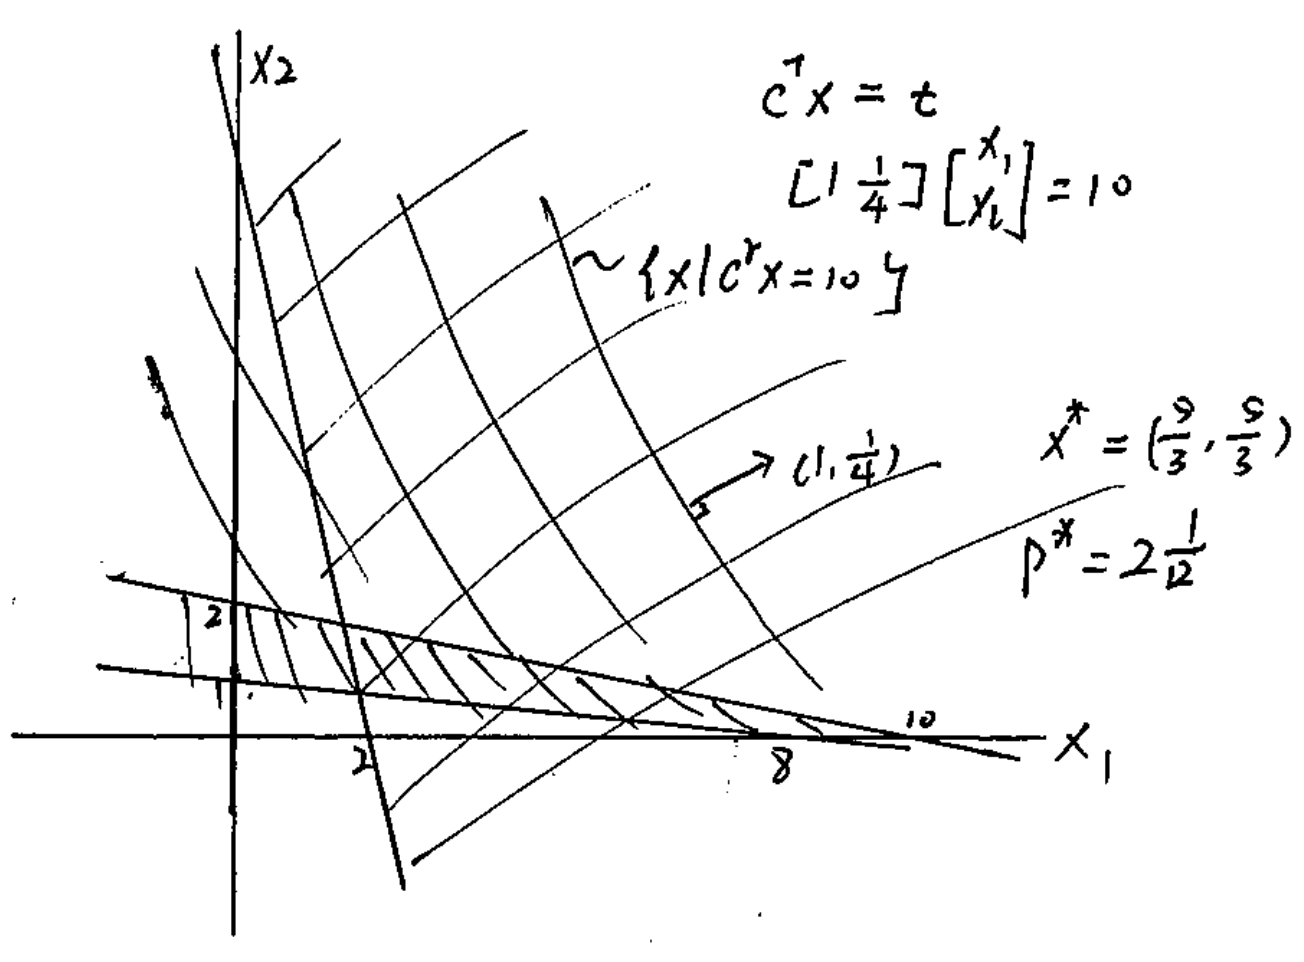
\includegraphics[width=2.1in,height=2.1in]{figures/ch06/figure5.png}
	%\caption{This is an inserted JPG graphic} 
	%\label{fig:graph} 
\end{figure}



\subsection{LP without contraints}

Consider the LPP does not have constraints, so we have
\begin{align*}
	p^* &= \min c^Tx+d\\
	x^* &= \arg \min_{x\in \reals^n} \,\,\, c^Tx+d
\end{align*}

\vspace{0.5cm}
Situation 1: $c = 0 \in \reals^n$
\begin{align*}
	p^* &= \min_{x\in \reals^n} \,\,\, d=d\\
	x^* &= \arg \min_{x\in \reals^n} \,\,\, d = \reals^n
\end{align*}

Situation 2: $c \neq 0 \in \reals^n$
\begin{align*}
	p^* &= -\infty\,\,\, \text{by convention if no minimum}\\
	x(\alpha) &= -\alpha c \,\,\, \alpha \geq 0\\
	c^Tx + d &= c^T(-\alpha c) + d = \alpha - \alpha c^Tc = \alpha - \alpha||c||^2_2\\
	x^* &\text{doesn't exist}
\end{align*}

Thus, for unconstrained LP we conclude that
$$
%\label{eq6}
p^*=\left\{
\begin{aligned}
d &  & \text{if } c=0 \\
-\infty &  & \text{otherwise}
\end{aligned}
\right.
%\label{eq6}
\qquad
x^*=\left\{
\begin{aligned}
\reals^n & &\text{if } c=0 \\
\text{doesn't exist} &  & \text{otherwise}
\end{aligned}
\right.
$$

Let's think about the geometry of cost function:
$$
F_0(x) =c^Tx + d
$$
where $F_0(x)$ is the objective function and it turns out that it is also an affine function.

Recall that the level set for $F_0(x)$, 
\begin{align*}
	c_{F_0}(t) &=\{ x\in \reals^n | F_0(x) = c^Tx + d = t \}\\
	&= \{x\in \reals^n | C^Tx = (t-d) \}
\end{align*}

Obviously, the level set for $F_0(x)$ defines a hyperplane, and when $t=d$ it defines a subspace(go through the origin). Let's consider two level sets, for $t_1$ and $t_2$,

\begin{figure}
	\centering
	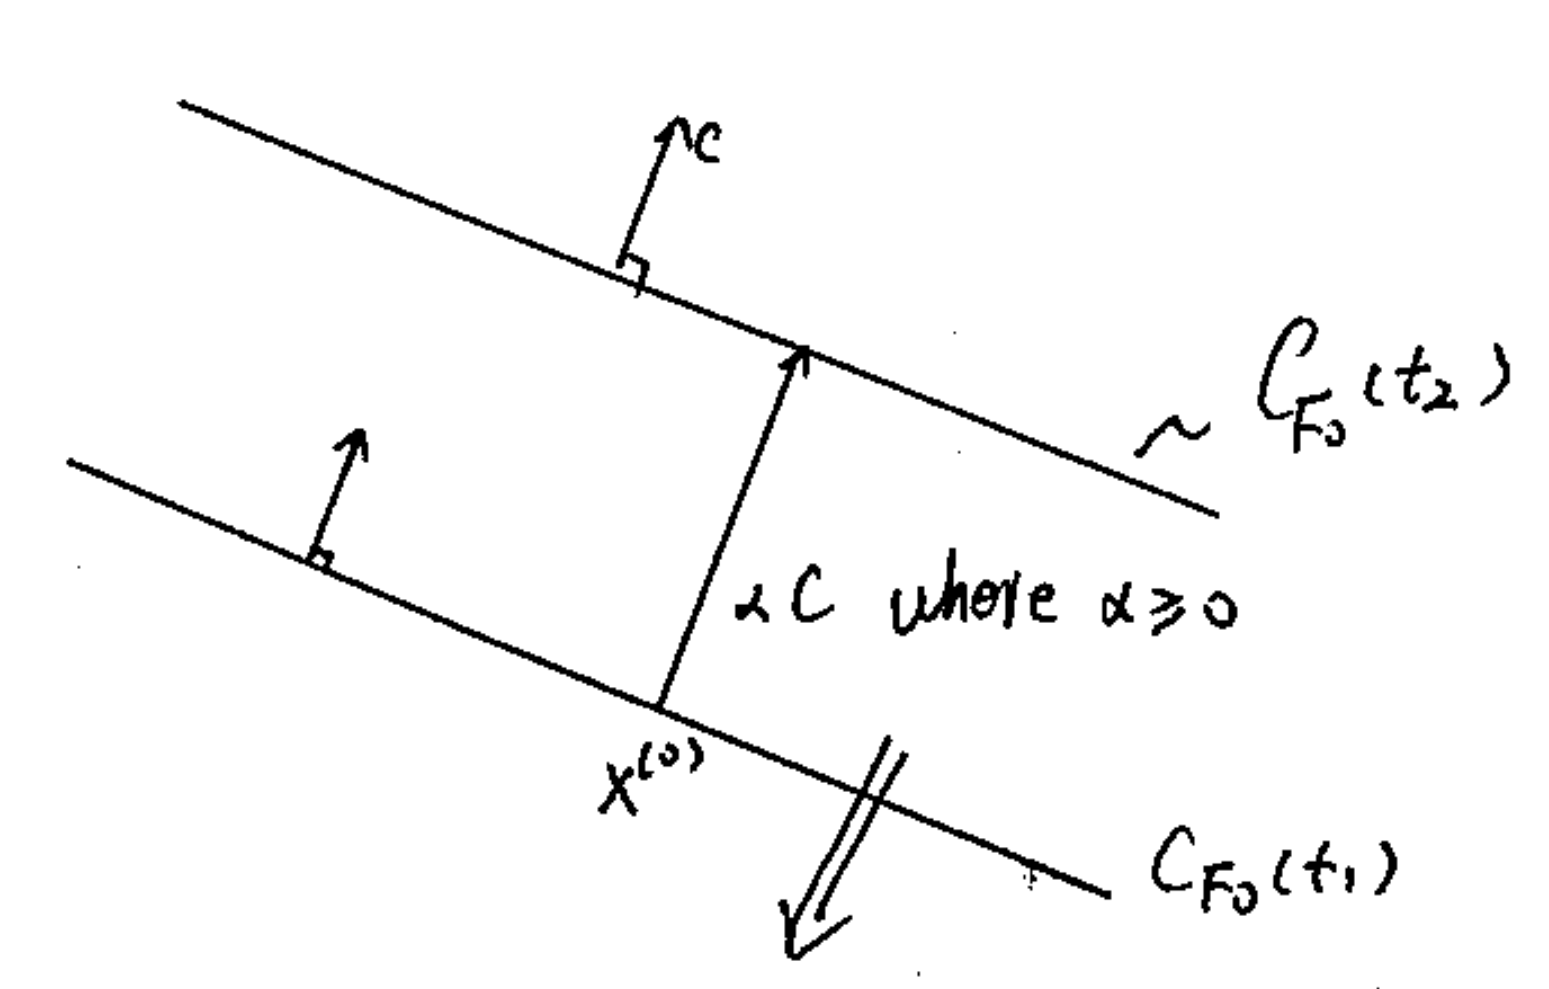
\includegraphics[width=2.1in,height=2.1in]{figures/ch07/figure1012_1.png}
	%\caption{This is an inserted JPG graphic} 
	%\label{fig:graph} 
\end{figure}

Note that $c$ is the normal vector to $x$. Let's find the relationship between $t_1$ and $t_2$:

Approach (1)
\begin{align*}
	t_2 &= c^T(x^{(0)}+\alpha c) + d\\
	t_1 &= c^Tx^{(0)} + d\\
	t_2 - t_1 &= [c^Tx^{(0)} + d + \alpha ||c||^2] - c^Tx^{(0)} = \alpha \Vert c \Vert^2
\end{align*}
So apparently $t_2>t_1$.

Approach (2)
\begin{equation*}
	\nabla F_0(x) =
	\begin{bmatrix}
		\frac{\sigma}{\sigma x_1}(c^Tx+d)\\
		\vdots\\
		\frac{\sigma}{\sigma x_n}(c^Tx+d)
	\end{bmatrix} = 
	\begin{bmatrix}
		c_1\\
		c_2\\
		\vdots\\
		c_n
	\end{bmatrix} = c
\end{equation*}

The gradient points out that the direction of $c$ is the direction of increase in $F_0(x)$. In fact, we could show that the direction of the gradient evaluated at a certain point, is the direction that the value of function increases more rapidly(remind yourself what you have learned in Calculus).

Hence, to minimize the objective function, we go in opposite direction of the gradient, that is, we should go as far as possible along the direction of $-c$ (unless $c=0$).


\vspace{0.5cm}
Now, let's turn back to LP with following constraints as we specified before:
\begin{align*}
	Ax &= b\\
	Gx &\leq h
\end{align*}

Interesting results and interpenetration for these two kind of constraints:

(1) $Ax=b$ (Equality contraints): force $x^*$ into an affine set
$$\{x\in \reals^n|Ax = b \} =  \cap^q_{i=1}\{x\in \reals^n|<\alpha^{(i)}, x> = b_i \}$$

(2) $Gx\leq h$ (Inequality contraints): force $x^*$ to be in an intersection of half-spaces
$$\{x\in \reals^n|Gx \leq h \} =  \cap^q_{i=1}\{x\in \reals^n| <g^{(i)}, x> \leq h_i \}$$

(3) The feasible set: intersection of half-spaces and hyperplanes
$$
S = \left(\cap^q_{i=1}\{x\in \reals^n | <\alpha^{(i)}, x> = b_i \}\right) \cap \left(\cap^m_{i=1}\{x\in \reals^n | <g^{(i)}, x> \leq h_i \}\right)
$$


A few remarks:
\begin{itemize}
	\item Concepts of polyhedron and polytape.
	
	\item Ax = b $\rightarrow$ $Ax \leq b$, $Ax \geq b$
\end{itemize}



\begin{example}
	\begin{align*}A &= 
		\begin{bmatrix}
			1 & 1
		\end{bmatrix}
		b = 
		\begin{bmatrix}
			2
		\end{bmatrix}\\
		G &= 
		\begin{bmatrix}
			-1 & 0\\
			0 & -1
		\end{bmatrix}
		h = 
		\begin{bmatrix}
			0\\
			0
		\end{bmatrix}\\
		Ax &= b \rightarrow x_1 + x_2 = 2\\
		Gx &\leq h \rightarrow x_1 \geq 0, x_2\geq 0
	\end{align*}
	
	
	\begin{figure}
		\centering
		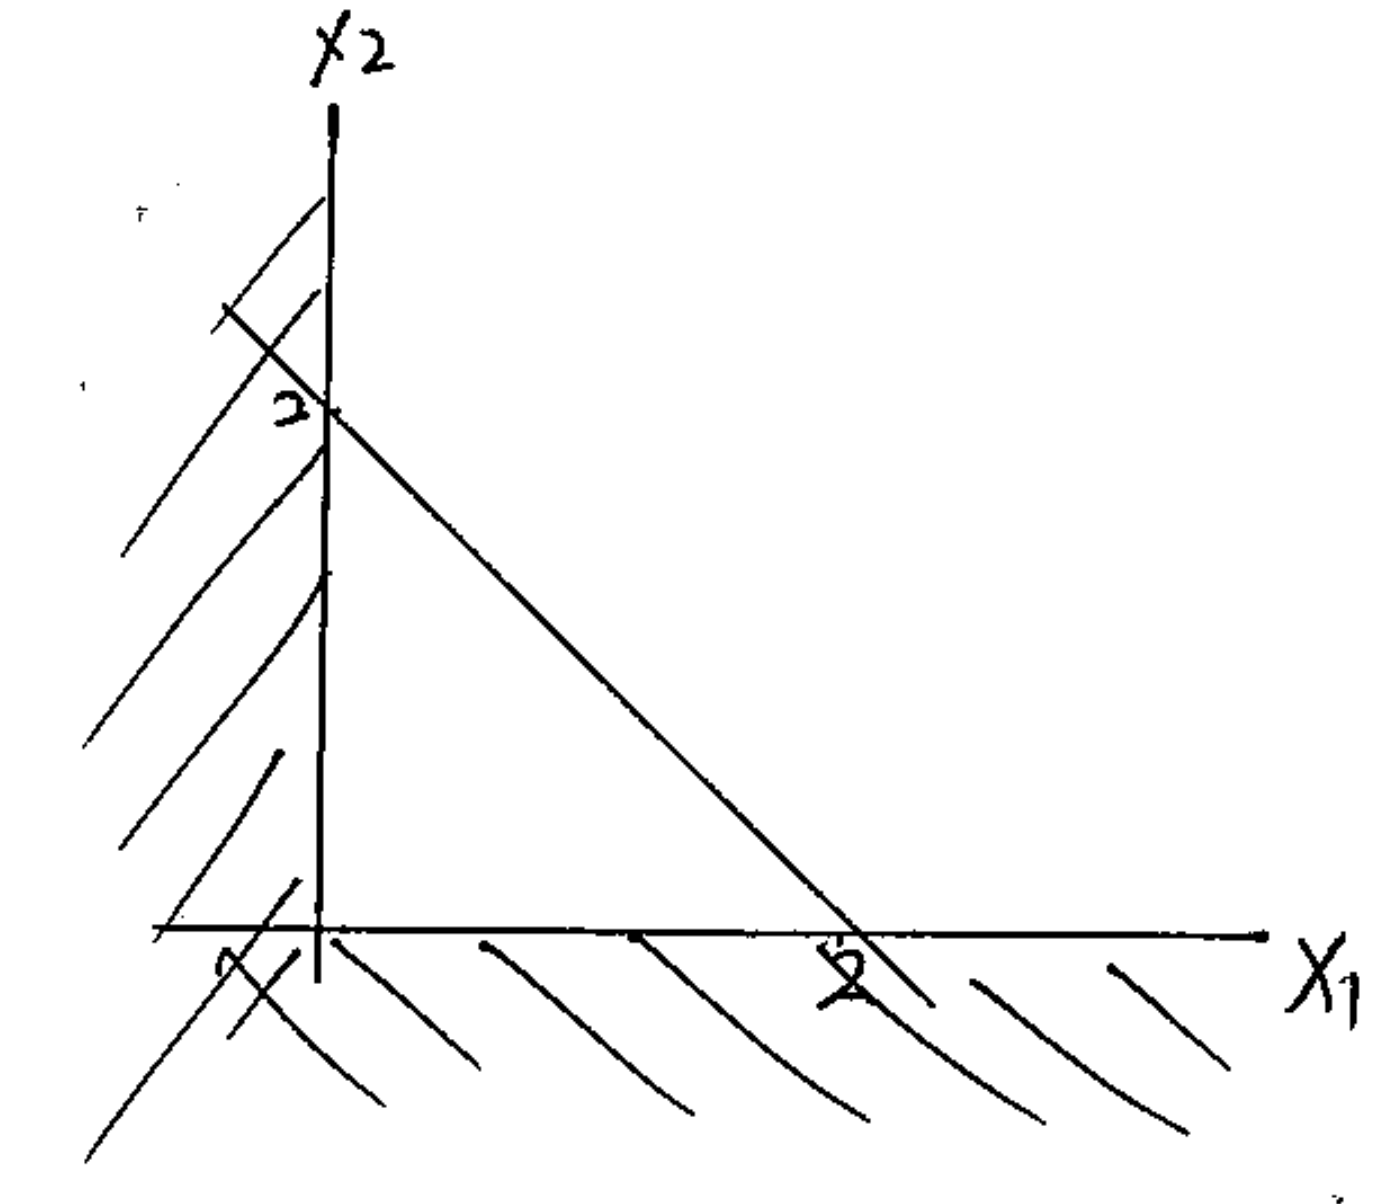
\includegraphics[width=2.1in,height=2.1in]{figures/ch07/figure1012_2.png}
		%\caption{This is an inserted JPG graphic} 
		%\label{fig:graph} 
	\end{figure}
\end{example}








\begin{example}
	Generally, equality constraints move you from a higher dimensional geometry in $\reals^n$ to a slice, which is a lower dimensional geometry. See the following example of losing 1 dimension per linearly independent constraint:
	
	
	\begin{align*}
		A =
		\begin{bmatrix}
			1&1&1
		\end{bmatrix}
	\end{align*}
	\begin{equation*}
		B= 
		\begin{bmatrix}
			1\\
		\end{bmatrix}
	\end{equation*}
	
	\begin{figure}
		\centering
		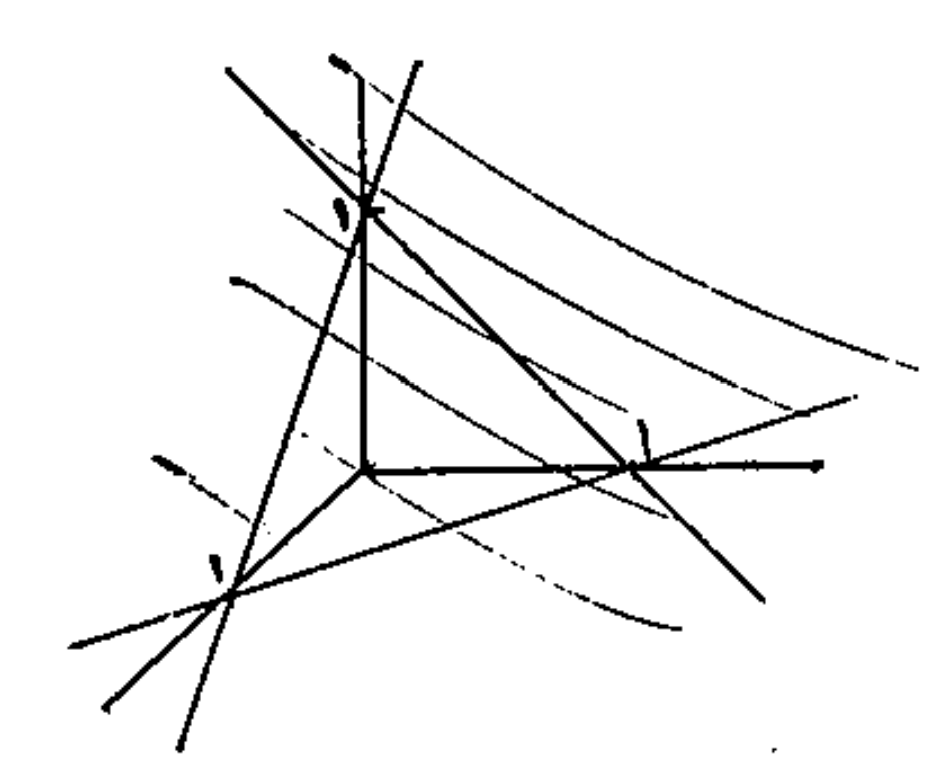
\includegraphics[width=2.1in,height=2.1in]{figures/ch07/figure1012_3.png}
		%\caption{This is an inserted JPG graphic} 
		%\label{fig:graph} 
	\end{figure}
\end{example}

\begin{example}
	In some cases, there may be no intersection between hyperplane:
	
	\begin{equation*}
		\begin{bmatrix}
			1&1\\
			1&1
		\end{bmatrix}
		\begin{bmatrix}
			x_1\\
			x_2
		\end{bmatrix}=
		\begin{bmatrix}
			1\\
			2
		\end{bmatrix}
	\end{equation*}
	
	\begin{figure}
		\centering
		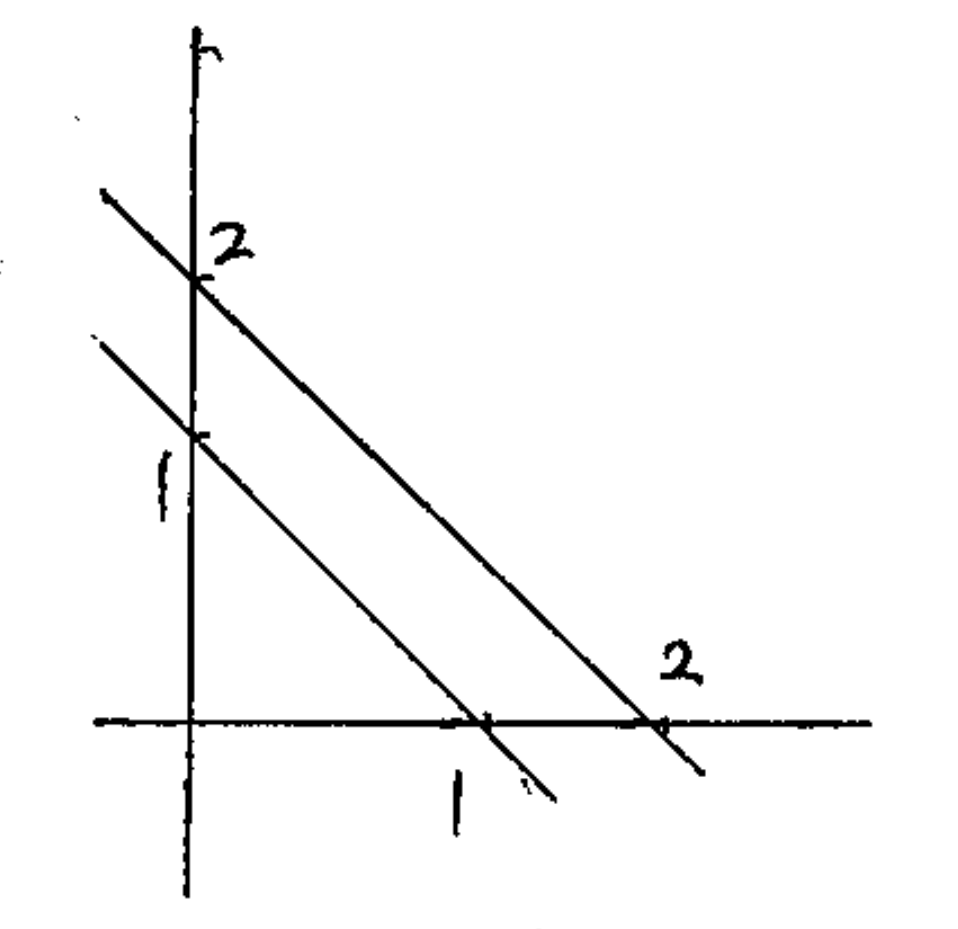
\includegraphics[width=2.1in,height=2.1in]{figures/ch07/figure1012_4.png}
		%\caption{This is an inserted JPG graphic} 
		%\label{fig:graph} 
	\end{figure}
	So the  feasible set is empty, $S = \emptyset$.
	
	\vspace{0.3cm}
	This situation may also happen with inequalities constraints:
	\begin{align*}
		\begin{bmatrix}
			-1&0\\
			1&0
		\end{bmatrix}
		\begin{bmatrix}
			x_1\\
			x_2
		\end{bmatrix}&\leq
		\begin{bmatrix}
			0\\
			-1
		\end{bmatrix}\\
		S &= \emptyset
	\end{align*}
	
\end{example}



\begin{example}
	Generally, to facilitate sketch will often just sketch inequity constraints:
	
	\begin{align*}
		\begin{bmatrix}
			-1 & 0\\
			0 & -1\\
			\frac{1}{2} & -1\\
			1 & 1
		\end{bmatrix}
		\begin{bmatrix}
			x_1\\
			x_2
		\end{bmatrix}
		&\leq 
		\begin{bmatrix}
			0\\
			0\\
			1\\
			3
		\end{bmatrix}\\
	\end{align*}
	
	So we have
	$$x_1 \geq 0$$
	$$x_2 \geq 0$$
	$$x_2 \geq -1 + \frac{1}{2}x_1$$
	$$x_2 \leq 3 - x_1$$
	
	Sketch the feasible set:
	
	\begin{figure}
		\centering
		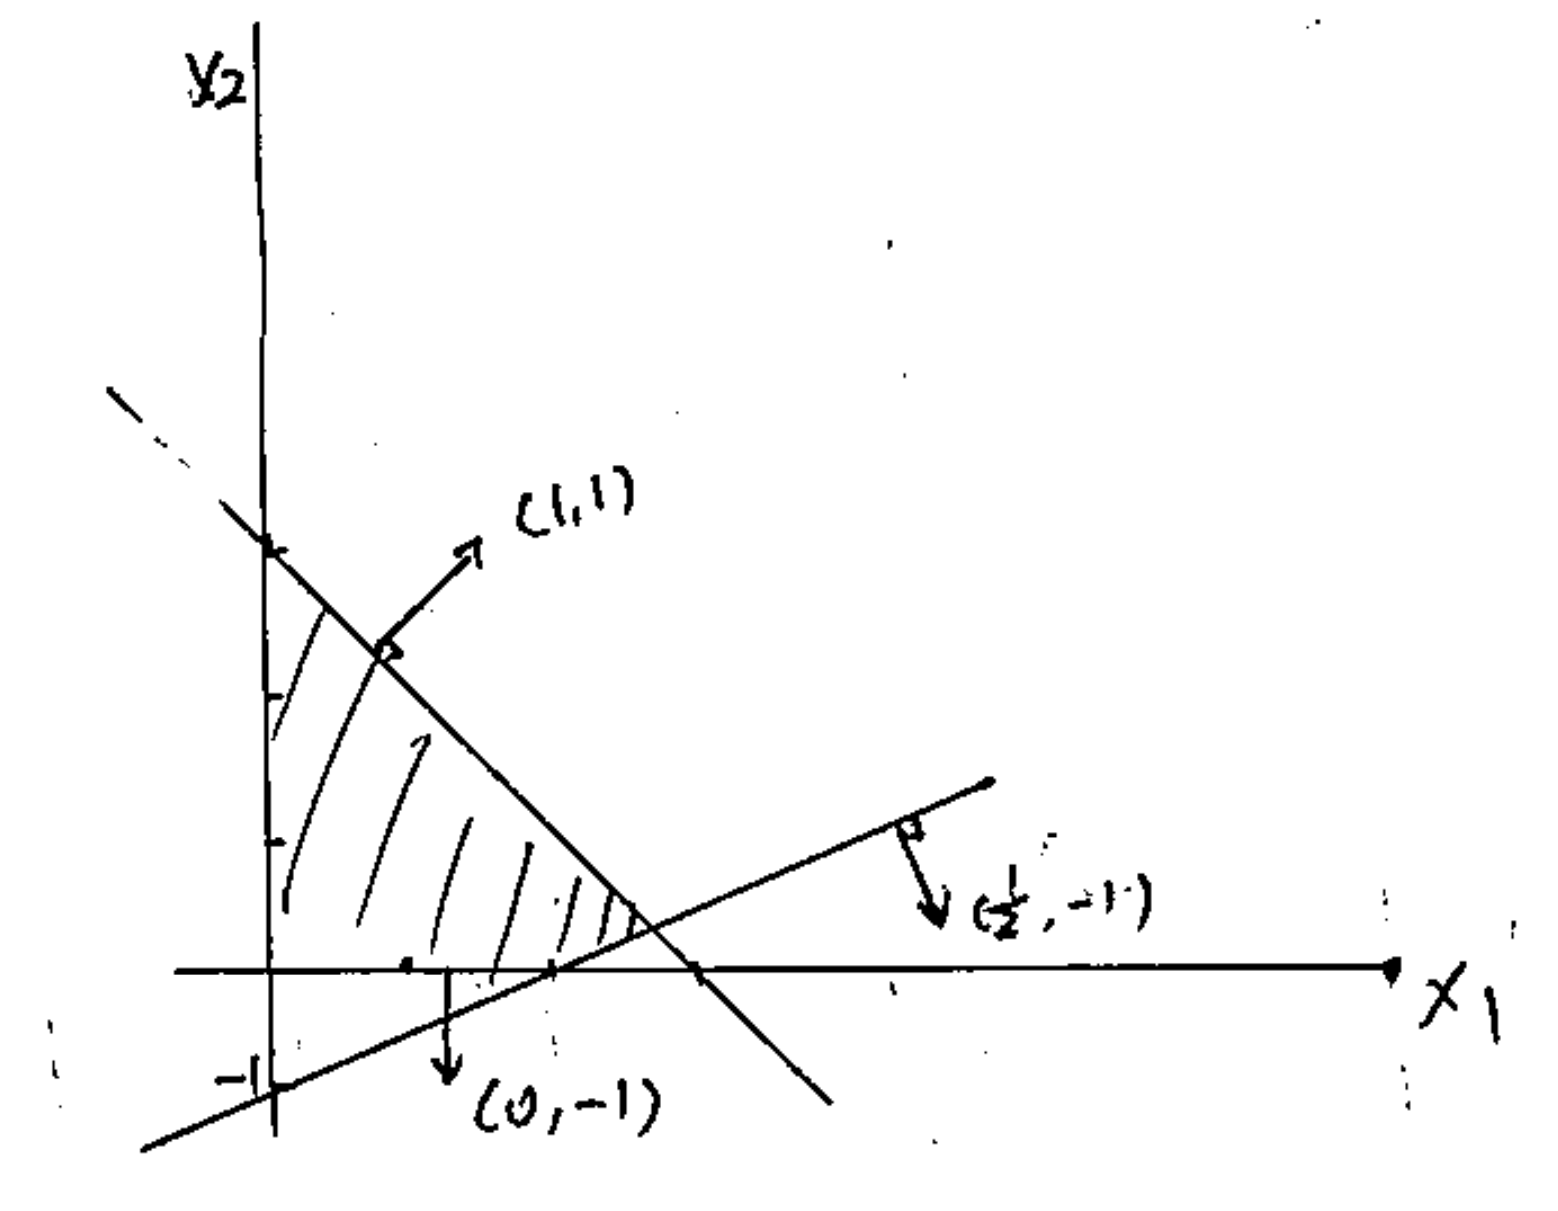
\includegraphics[width=2.1in,height=2.1in]{figures/ch07/figure1012_5.png}
		%\caption{This is an inserted JPG graphic} 
		%\label{fig:graph} 
	\end{figure}
\end{example}

The rows of matrix $G$ are the normal directions of the hyperplanes that define the half-spaces, and the normal directions point outward from the feasible set.


\begin{example}
	Let's combine all these things together, liner objective function, linear equality constraints and linear inequity constraints.
	
	\begin{figure}
		\centering
		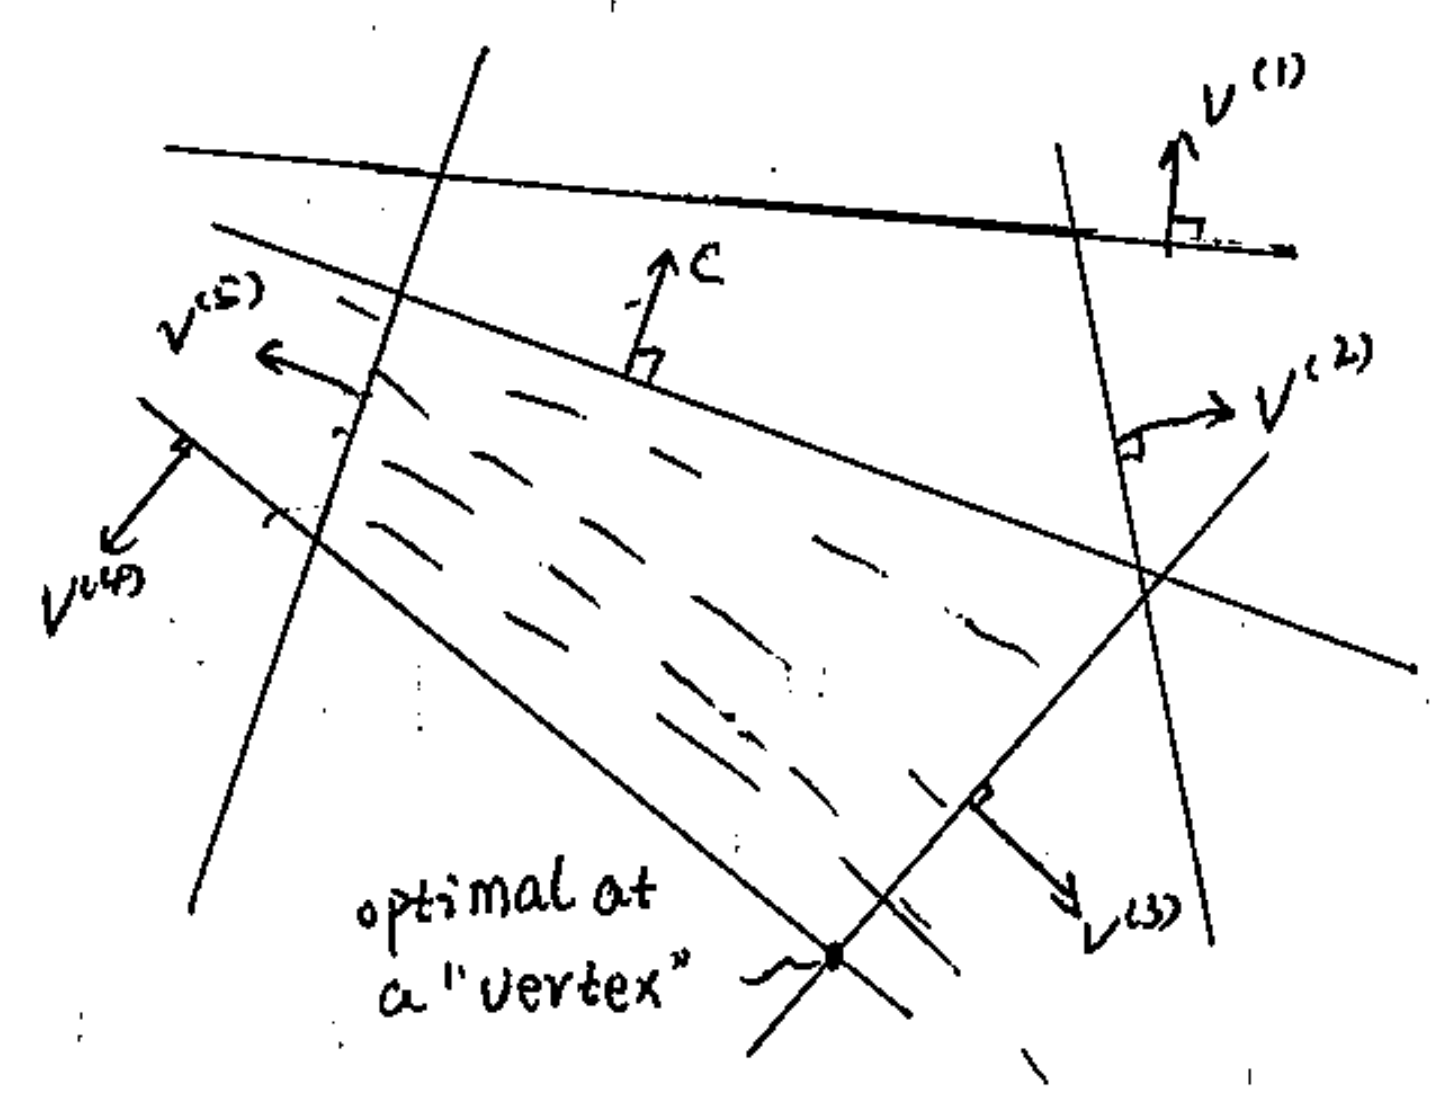
\includegraphics[width=2.1in,height=2.1in]{figures/ch07/figure1012_6.png}
		%\caption{This is an inserted JPG graphic} 
		%\label{fig:graph} 
	\end{figure}
	
	What's optimum? Looks like $x^*=v^{(3)}$.
	
	
	\vspace{0.5cm}
	We may also have a facet with the feasible set 
	$$S = \{x\in \reals^3 | x_1 +x_2+x_3 = 1, x_1 \geq 0, x_2\geq 0,x_3\geq 0\}$$
	
	
	\begin{figure}
		\centering
		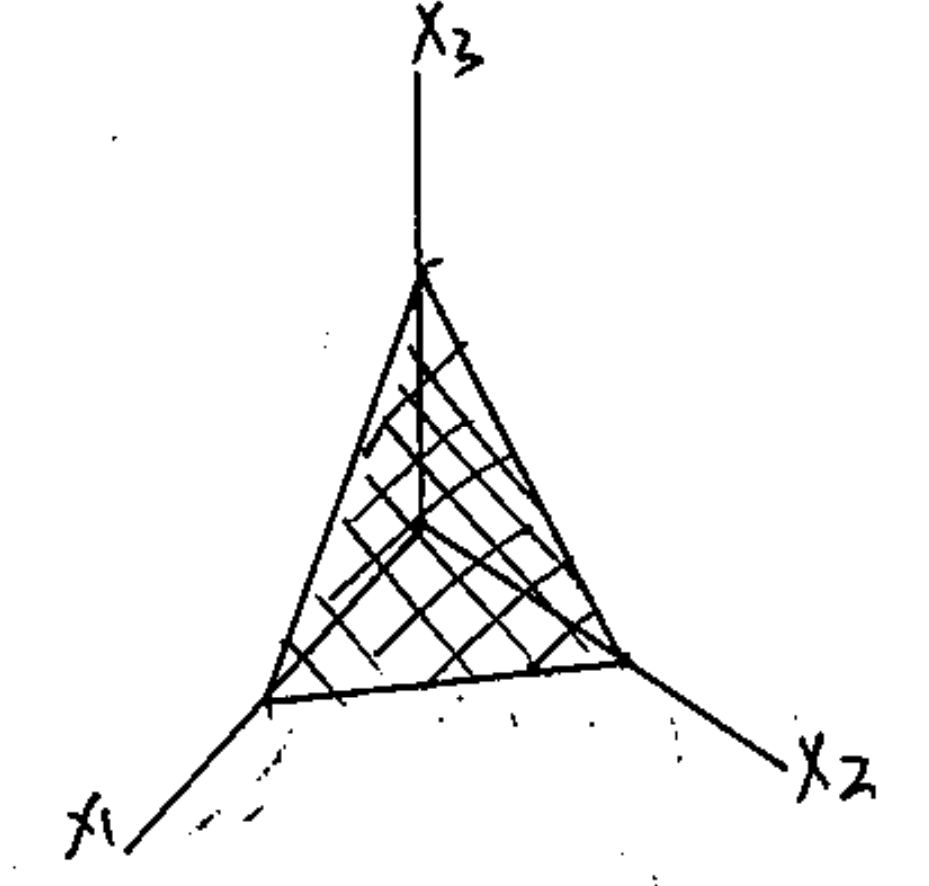
\includegraphics[width=2.1in,height=2.1in]{figures/ch07/figure1012_7.png}
		%\caption{This is an inserted JPG graphic} 
		%\label{fig:graph} 
	\end{figure}
	
	So there are various possibilities here for $p^*$ and  $x^* $:
	
	\begin{itemize}
		\item 1) $x^*$ is unique, $p^*$ finite
		
		\item 2) $x^*$ is not unique, $p^*$ finite. 
		
		\item 3) There is no $x^*$:
		
		\quad a) $S = \emptyset$ (Feasible set is empty), constraint $p^* = \infty$. So we say that this LP problem is infeasible.
		
		\quad b) $S$ is unbounded \& no minimum, constraint $p^* = -\infty$
	\end{itemize}
	
	
	\begin{figure}
		\centering
		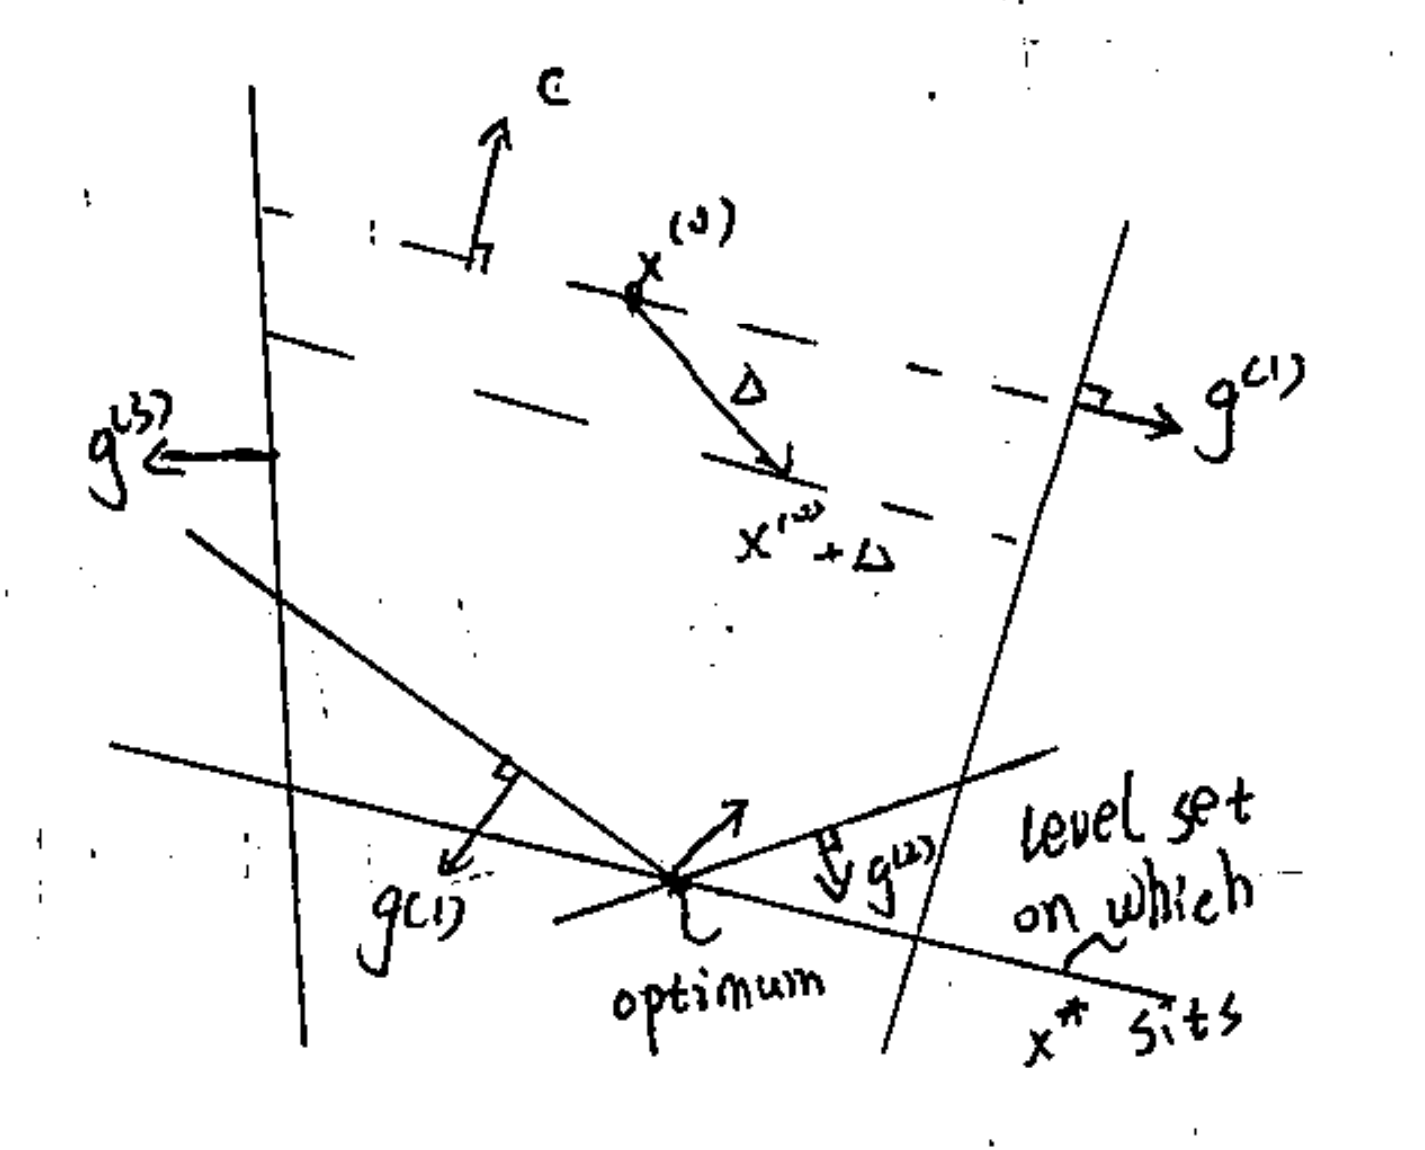
\includegraphics[width=2.1in,height=2.1in]{figures/ch07/figure1012_8.png}
		%\caption{This is an inserted JPG graphic} 
		%\label{fig:graph} 
	\end{figure}
	
	Active constraints: An optimal solution that lies at the intersection point of two constraints causes both of those constraints to be considered active
	
	Inactive constraints: If any of the constraint lines do not pass through the optimal point, those constraints are called inactive.
	
	In this example(see picture above) constraints g(1) and g(2) are active at optimum.
	
	Note that, we could improve(decrease) the cost if:
	$$c^T(x^{(0)} + \bigtriangleup) + d < c^Tx^{(0)} + d$$
	That is, $\langle c, \bigtriangleup\rangle < 0$, the angle between displacement vector $\bigtriangleup$ and normal vector $c$ is an obtuse angle(see the picture above).
\end{example}





\vspace{0.5cm}
Some observations:
\begin{itemize}
	\item If you are at a vertex(doesn't have to be optimum). 
	
	\item Any "move" that keeps you feasible must also let you move into the feasible set 
	
	$\rightarrow$ opposite vector that define active constraints.
	
	\begin{equation*}
		v - \alpha g^{(1)} - \beta g^{(2)}, \,\,\, \alpha, \beta \geq 0
	\end{equation*}
	
	\item Are these any choices of $\alpha, \beta$ that decrease the cost?
	\begin{align*}
		c^T(v - \alpha g^{(1)} - \beta g^{(2)}) + d &\leq c^Tx + d\\
		-\alpha \langle c, g^{(1)}\rangle  - \beta \langle c, g^{(2)}\rangle &\leq 0
	\end{align*}
\end{itemize}

If:

1) $\langle c, g^{(1)}\rangle < 0$

2) $\langle c, g^{(2)}\rangle < 0$

no more into feasible set will decrease the cost.\\ 

\vspace{0.5cm}
Condition for optimality:

A feasible vertex $v$: $v\in\{x|Gx \leq h \}$ is an optimal solution to LP with cost $F_0(x) = c^Tx + d$ if $c^Tg^{(i)} < 0$, $\forall i\in$ active set.\\

\begin{figure}
	\centering
	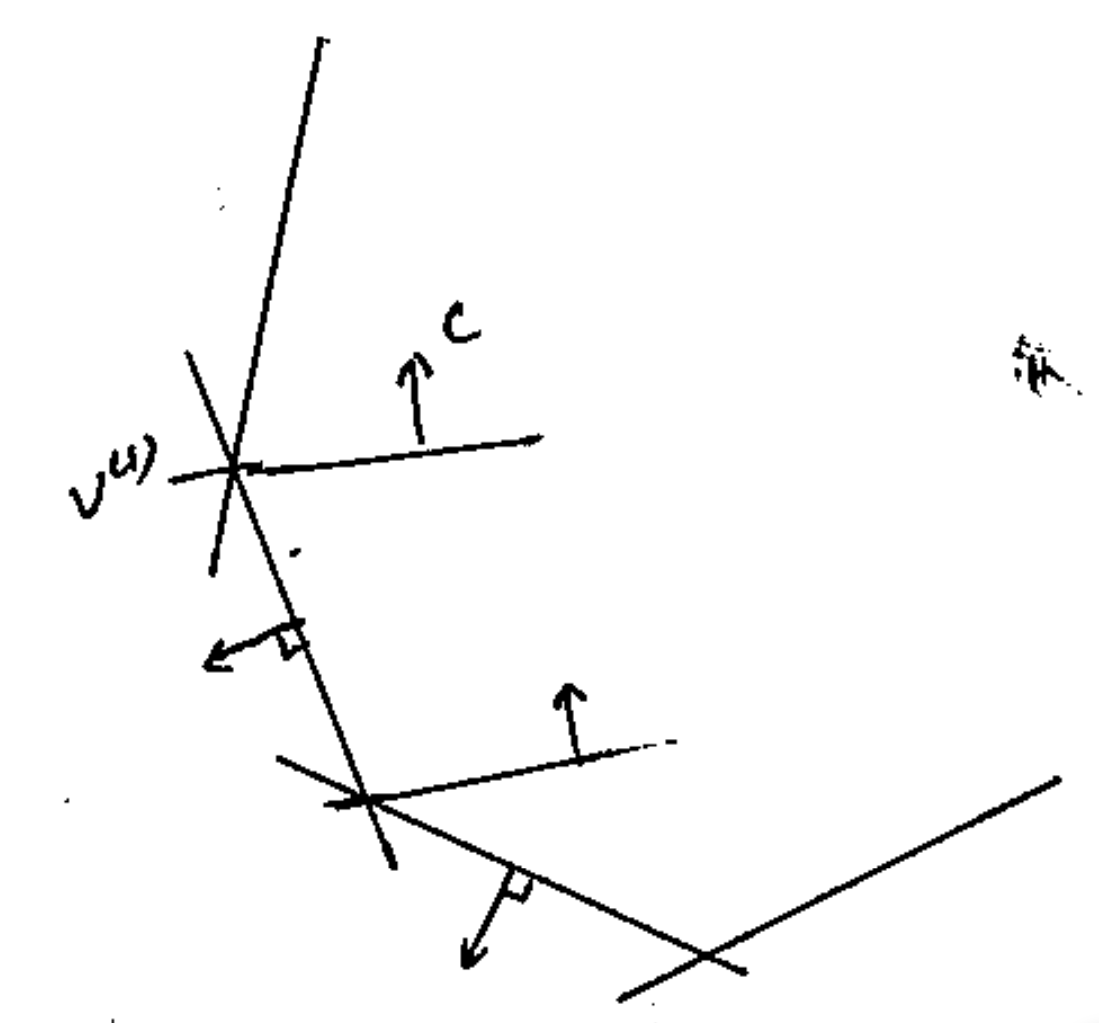
\includegraphics[width=2.1in,height=2.1in]{figures/ch07/figure1012_9.png}
	%\caption{This is an inserted JPG graphic} 
	%\label{fig:graph} 
\end{figure}


\subsection{Simplext Algorithm}
Simplex algorithm:
\begin{itemize}
	\item 1) Start from a feasible vertex;
	
	\item 2) Identify direction of cost decrease along an edge;
	
	\item 3) Move on that direction until any further more would violate a previously inactive constraints.
	
	\item 4) Stop + add that new constraint(s) to active set.
	
	\item 5) Repeat
\end{itemize}




%\begin{equation*}
%\{x|Gx\leq h \}
%\end{equation*}


%\begin{figure}
%	\centering
%	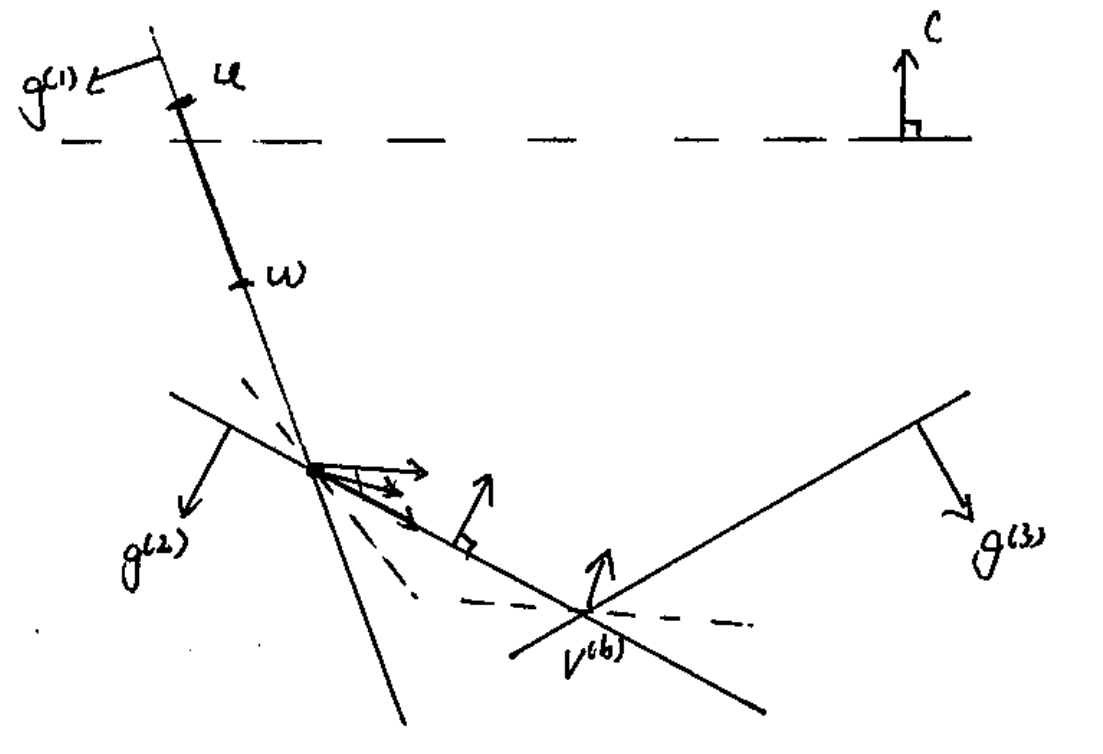
\includegraphics[width=2.1in,height=2.1in]{figures/ch07/figure1016_1.png}
%\caption{This is an inserted JPG graphic} 
%\label{fig:graph} 
%\end{figure}


%If $x =v^{(a)}$, constraints, constraints 1\&2 active, 3 is inactive.

%\begin{align*}
%<g^{(1)}, v^{(a)}> &= h_1\\
%<g^{(2)}, v^{(a)}> &= h_2\\
%<g^{(3)}, v^{(a)}> &< h_3
%\end{align*}

%At $x = v^{(b)}$, constraints 2\&3 active, 1 is inactive.\\

%1) Define a vertex $v$:

%\begin{itemize}
%	\item a) $v\in S$ is a vertex if cannot express $v = \lambda u +(1-\lambda)w$, $u, w\in S$, $\lambda \in [0,1]$

%	\item b) There exists a cost vector $c\in \reals^n$ s.t. $v$ is unique solution to an LP with cost vector $c$.

%	\item c) Algebraic characterization of vertices in terms of $A, b, G, h$. $S = \{x|Ax \leq b, Gx\leq h \}$
%\end{itemize}



%2) Define / Find directions along edges of polyhedron that keep you in the feasible set.

%3) How far can you go in direction that decrease cost until "leave" feasible set?


\begin{example}
	Consider the problem:
	\begin{align*}
		&min \Vert Ax - b\Vert_{\infty}\\
		&s.t. Gx \leq h
	\end{align*}
	
	Recall that $\Vert u\Vert_{\infty} = max_{i\in [n]}|u_i|$,
	\begin{figure}
		\centering
		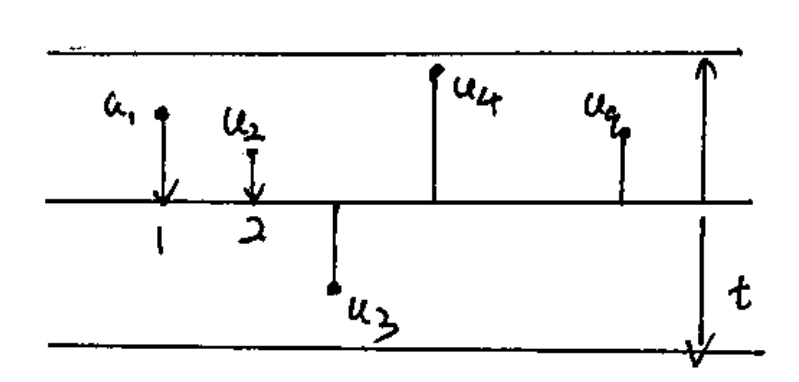
\includegraphics[width=2.1in,height=2.1in]{figures/ch07/figure1016_2.png}
		%\caption{This is an inserted JPG graphic} 
		%\label{fig:graph} 
	\end{figure}
	
	Introduce a helper(auxiliary) variable $t\in \reals$ which corresponding to the value of the norm, so the we convert the original problem into following problem:	
	\begin{align*}
		min &\qquad t\\
		s.t. &Ax - b\leq t\textbf{1}\\
		&Ax - b\geq (-t)\textbf{1}\\
		&Gx \leq h
	\end{align*}
\end{example}


\begin{example}
	Consider the problem:
	\begin{align*}
		min_x &||Ax - b||_1, \,\,\,\,\, A\in \reals^{q\times n}\\
		s.t. &Gx\leq h
	\end{align*}
	\begin{figure}
		\centering
		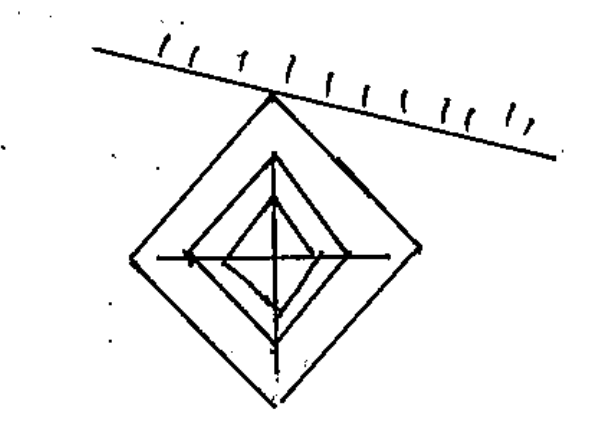
\includegraphics[width=2.1in,height=2.1in]{figures/ch07/figure1016_3.png}
		%\caption{This is an inserted JPG graphic} 
		%\label{fig:graph} 
	\end{figure}
	
	Recall the definition of $L_1$ norm:
	\begin{equation*}
		||u||_1 = \sum^q_{i=1} |u_i|
	\end{equation*}
	
	%	\begin{figure}
	%		\centering
	%		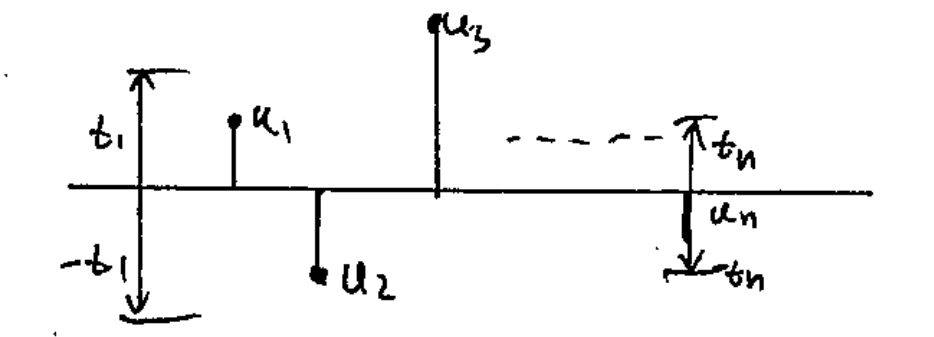
\includegraphics[width=2.1in,height=2.1in]{figures/ch07/figure1016_4.png}
	%		%\caption{This is an inserted JPG graphic} 
	%		%\label{fig:graph} 
	%	\end{figure}
	
	Let's introduce the helper vector $t\in \reals^q$,
	\begin{align*}
		min_{x,t} &\sum^q_{i=1}t_i\\
		s.t. \,\,\,\,\,&Gx \leq h\\
		&Ax -b \leq t\\
		&Ax -b \geq -t
	\end{align*}
	
\end{example}



\begin{example}
	Consider following problem:
	\begin{align*}
		min \,\,\, max_{i\in [q]} &(c^{(i)^T}x + d_i)\\
		s.t. &Gx\leq h
	\end{align*}
	This case is similar to the $L_\infty$ norm case due to the inner max function, but it is one-sided(no lower bound). So we could convert the original one to the following:
	\begin{align*}
		min  &\qquad t\\
		s.t. &(c^{(i)^T}x + d_i)\leq t,\,\,\,\,\, \forall i\in [q]\\
		&Gx\leq h
	\end{align*}
	\begin{marginfigure}
		\centering
		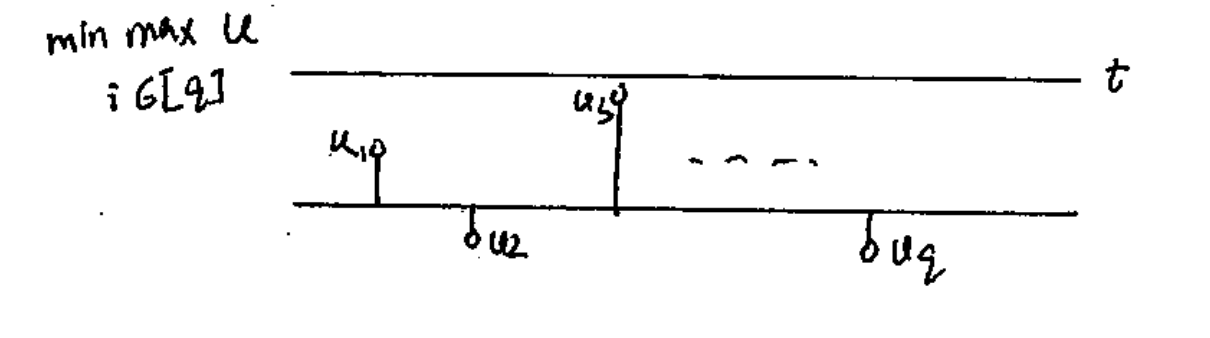
\includegraphics[width=2.1in,height=2.1in]{figures/ch07/figure1016_5.png}
		%\caption{This is an inserted JPG graphic} 
		%\label{fig:graph} 
	\end{marginfigure}
\end{example}

Remark:

In above three examples, the decision variables in initial formulation are $x\in \reals^n$, but in reformulation they become:

Example 7.6: $(x, t) \in \reals^n \times \reals$

Example 7.7: $(x, t) \in \reals^n \times \reals^n$

Example 7.8: $(x, t) \in \reals^n \times \reals$



\begin{example}
	Finding the largest $L_2$ ball that fits in a polytope.
	
	Let $p = \{x\in \reals^n| Gx\leq h \}$,
	
	\begin{figure}
		\centering
		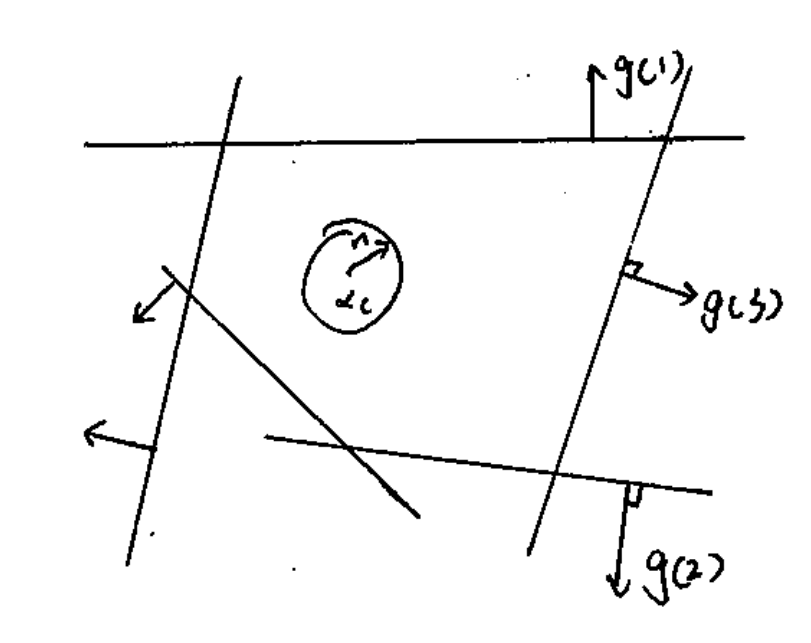
\includegraphics[width=2.1in,height=2.1in]{figures/ch07/figure1016_6.png}
		%\caption{This is an inserted JPG graphic} 
		%\label{fig:graph} 
	\end{figure}
\end{example}

It turns out that, this problem can be formulated as an LP problem. \

Note that:
\begin{itemize}
	\item A sphere is fully parameterized by its center $x_c$ and its radius $r$
	
	\item A sphere $(x_c, r)$ fits in $p$ if: $x_c + u \in p$, $\forall u \,\,\, s.t. ||u||_2\leq r$
\end{itemize}

\vspace{0.3cm}
Now, let's formulate as an LP. To accomplish this, observe that 

$x_c+u \in p$ means that $g^{(i)^T}(x_c + u) \leq h_i,\,\,\, \forall i\in [q]$, $\forall u$ s.t. $||u||_2\leq r$.

\vspace{0.2cm}
Examine the constraint $g^{({i})^T}x_c + g^{({i})^T}u \leq h_i$ at a time:

As for $g^{({i})^T}u$, what's the direction of $u$ in order to make this term large as possible? It turns out, $u$ must be aligned with $g^{(i)}$, the same direction with $g^{(i)}$.

Furthermore, what's the value of $u$ that is aligned with $g^{(i)}$ and satisfies  $\vert u\vert_2=r?$ It should be:
$$u^*=\frac{g^{(1)}}{||g^{(1)}||}r$$


So, if the following is satisfied:
$$g^{(i)^T}[x_c + u^*] \leq h_i$$\
Then constraint $i$ will be satisfied for all $u$ such that $\vert u\vert \leq r$.

Substituting in $u^*$, the constraints become:
$$g^{(i)^T} x_c + \Vert g^{(i)}\Vert_2 r\leq h_i$$
Note that the constraint is linear in $x_c$ and $r$.

The problem of finding the largest sphere becomes the following:
\begin{align*}
	\max \quad & r\\
	s.t.\quad &g^{(i)^T}x_c + r ||g^{(i)}||_2\leq h_i \qquad \forall i\in [q]
\end{align*}


Remarks:

(1) Optimal value $(x_c, r)\in \reals^{n+1}$.

(2) $x_c$ is a variable that does not enter the objective.

(3) Possibly no solution if $p$ is an empty set.

(4) Constraints and objective are linear in optimal variable so it is an LP problem.

(5)Transformed some quadratic-like problem (quadratic as a sphere is involved) into an LP, because we were able to identify which direction of $u$ the worst case for each constraint.























\newpage

\section{Quadratic program(QP)}

\begin{align*}
p^* = min_{x\in \Re^n} &\frac{1}{2}x^THx + c^Tx + d\\
s.t. \,\,\, &Ax = b\\
&Gx \leq h
\end{align*}

\begin{figure}
	\centering
	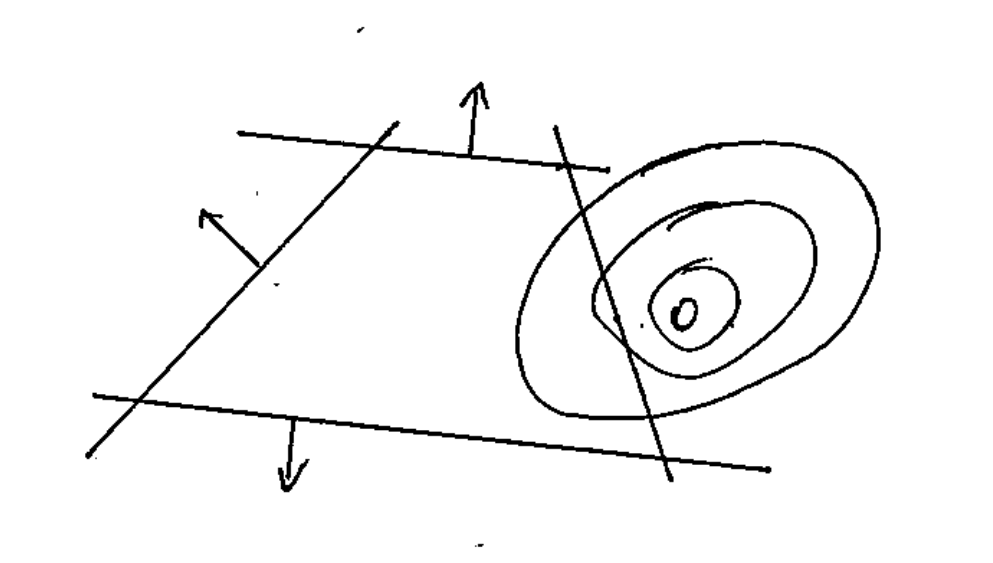
\includegraphics[width=2.1in,height=2.1in]{figures/ch07/figure1016_7.png}
	%\caption{This is an inserted JPG graphic} 
	%\label{fig:graph} 
\end{figure}
%Above are notes for Oct14


\section{10.16}

%Below are notes for Oct16

\begin{align*}
p^* = min_{x\in \Re^n}\,\,\,\,\, &\frac{1}{2}x^THx + c^Tx + d\\
 s.t.\,\,\,\,\, &Ax = b\\
 &Gx\leq h
\end{align*}


\begin{figure}
	\centering
	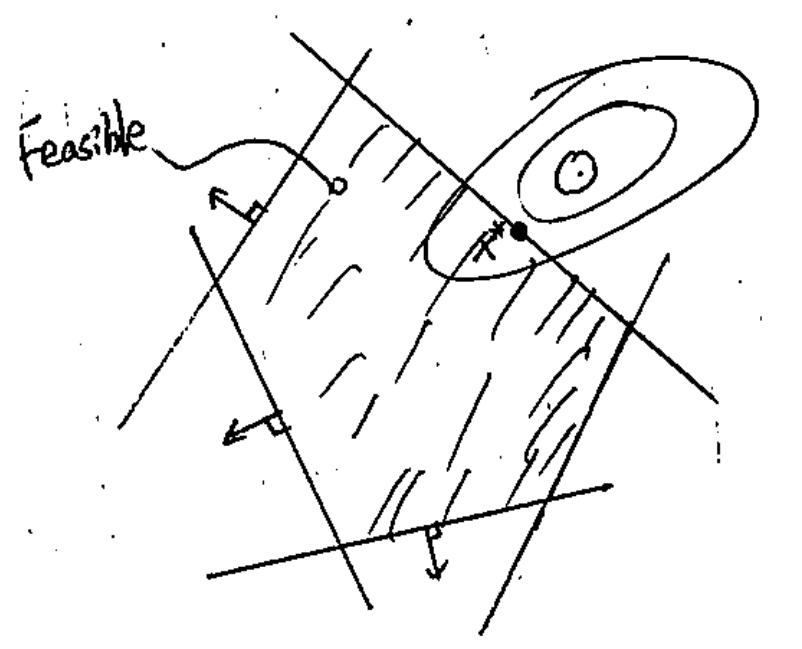
\includegraphics[width=2.1in,height=2.1in]{figures/ch07/figure1016_a.png}
	%\caption{This is an inserted JPG graphic} 
	%\label{fig:graph} 
\end{figure}

\subsection{Least squares}
\begin{align*}
||Ax - y||_2^2 &= (Ax - y)^T(Ax - y)\\
&= x^TA^TAx - 2y^TAx + y^Ty\\
&= \frac{1}{2}x^T(2A^TA)x - 2y^TAx + ||y||_2^2
\end{align*}

Note: Cannot always manipulate objective of a QP into form of objective of a LS problem.\\

\subsection{Equality constrained QPs}

\begin{align*}
p^* = min_{x\in \Re^n}\,\,\,\,\, &\frac{1}{2}x^THx + c^Tx + d\\
s.t.\,\,\,\,\, &Ax = b
\end{align*}


\begin{figure}
	\centering
	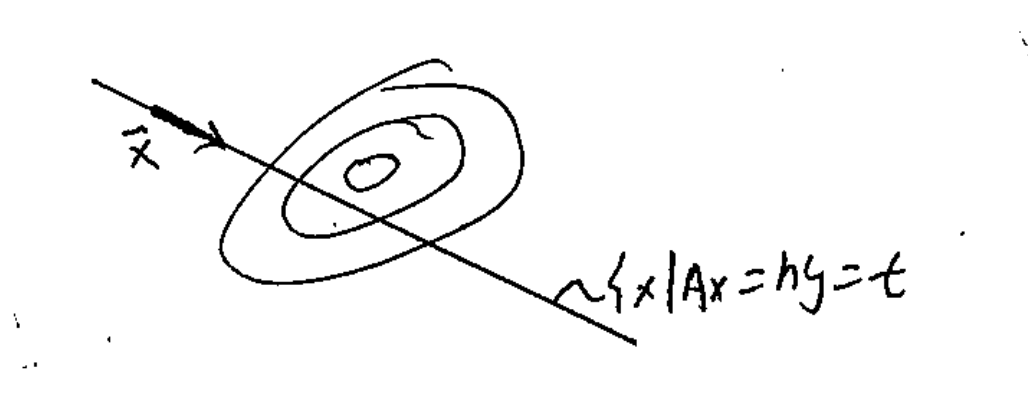
\includegraphics[width=2.1in,height=2.1in]{figures/ch07/figure1016_b.png}
	%\caption{This is an inserted JPG graphic} 
	%\label{fig:graph} 
\end{figure}

\begin{equation*}
\mathcal{A} =\{x | x = \bar{x} + \xi,\,\,\, \text{where } \xi \in N(A) \}
\end{equation*}

Let N be a basis for $N(A)$, can express $\xi \in N(A)$ as $\xi = Nz$ where $z\in \Re^k$, $k =dim(N(A)) \leq n$


Substitute this expression for any feasible $x$ into objective $F_0(\cdot)$


\begin{align*}
F_0(x) &= F_0(\bar{x} + \xi) = F_)(\bar{x} + Nz)\\
&= \frac{1}{2}(\bar{x} + Nz)^TH(\bar{x}+Nz) + c^T(\bar{x} + Nz) + d\\
&= \frac{1}{2}z^T[N^THN]z + [c^TN + \bar{x}^THN]z + [\frac{1}{2}\bar{x}^TH\bar{x} + c^Tx + d] \\
\end{align*}

\begin{equation*}
p^* = min_{z\in \Re^k}\,\,\,\,\, \frac{1}{2}z^T\tilde{H}z + \tilde{c^T}z + \tilde{d}
\end{equation*}

$\rightarrow$ lower-dimensional optimization problem $k =dim(N(A)) \leq n $

$\rightarrow$ still a QP, but an unconstrained QP.



\begin{example}{Markowitz Partfolio optimization}
	"Mean/variance" analysis
	
	\begin{itemize}
		\item Minimize amount of variance in returns for a fixed level of (expected) returns
		
		\item Harry Markowitz(1990 Nobel Prize)
	\end{itemize}
	
	\textbf{Model}: There are n stock, single investment period\\
	
	\textbf{Task}:
	
	\begin{itemize}
		\item Design an investment strategy $p\in \Re^n$
		
		\item $p_i = $ amount/proportion of wealth invested in stock $i$
		
		\item $\sum^n_{i=1}p_i = 1$, "all-in" invest all your money
		
		\item $p_i \geq 0$, "long" positions(no "short time")
		
		\item Wealth normalized to 1
	\end{itemize} 
	
	\textbf{Returns}:
	
	\begin{itemize}
		\item $x\in \Re^n$
		
		\item $x_i$ = return on $i^th$ stock in period if must 1RMB in stock: get $x_i$RMB back.
	\end{itemize} 
	
	
	\textbf{Probabilistic model on returns}:
	
	\begin{itemize}
		\item Expected returns: $\bar{x_i} = \mathbb{E}[x_i]$(known)
		
		\item Your return (random) is $\sum^n_{i=1}p_ix_i = p^Tx$
		
		\item Your expected value $\mathbb{E}[\sum^n_{i=1}p_ix_i] = \sum^n_{i=1}p_i\mathbb{E}[x_i] = \sum^n_{i=1}p_i\bar{x_i} = p^T\bar{x}$
		
		\item variance in returns:
		
		\begin{align*}
		var(p^Tx) &=\mathbb{E}[(p^Tx - p^T\bar{x})^2]\\
		&= \mathbb{E}[(p^T(x - x^T))^2]\\
		&= \mathbb{E}[p^T(x - \bar{x})(x - \bar{x})^Tp]\\
		&= p^T\mathbb{E}[(x - \bar{x})(x - \bar{x})^T]p\\
		&= p^T\Sigma p
		\end{align*}
	\end{itemize}
	
	
	
	
	
	
	
	
	

	
	Given mean returns $\bar{x}$ and covariance matrix of returns $\Sigma \in \Re^{n\times n}$. Design $p$ to minimize "risk" subject to same minimal returns.:
	
	\begin{align*}
	min_{p\in \Re^n}\,\,\,\,\, &p^T\Sigma p\\
	s.t. \,\,\,\,\,&p^T\bar{x}\geq r_{min}\\
	&\textbf{1}^Tp = 1\\
	&p\geq 0
	\end{align*}
\end{example}




\begin{align*}
p^* = min_{x\in \Re^n}\,\,\,\,\, &\frac{1}{2}x^THx + x^Tx + d\\
s.t.\,\,\,\,\, &Ax = b\\
&Gx\leq h
\end{align*}

Discuss geometry of objective

Discuss geometry of feasible set

1) w.l.o.g assume $H\in S^n$, 

\begin{align*}
x^THx &=\frac{1}{2}[x^THx + x^TH^Tx]\\
 &= \frac{1}{2}x^T(H+H^T)x
\end{align*}

Hence always consider $H$ symmetric.\\



\subsection{Symmetric matrices}

1) Eigenvalues: purely real eigenvalues (can sort)

2) Eigenvectors: can always be chosen $\perp$ and can always diagonalize

\begin{equation*}
H = \mathcal{U}\Lambda \mathbb{U}^T  = \sum^n_{i=1}\lambda_iu^{(i)}u^{(i)^T}
\end{equation*}

For 3 cases:

\begin{equation*}
F_0(x) = \frac{1}{2}x^THx + c^Tx + d
\end{equation*}

\begin{itemize}
	\item A) $H\in S^n$ but not PSD
	
	\begin{equation*}
	H = 
	\begin{bmatrix}
	1&0\\
	0&-2
	\end{bmatrix}
	\end{equation*}
	
	\item B) $H\in S^n_+$ but not PD
	\begin{equation*}
	H = 
	\begin{bmatrix}
	1&0\\
	0&0
	\end{bmatrix}
	\end{equation*}
	
	\item C) $H\in S^n_{++}$
	\begin{equation*}
	H = \begin{bmatrix}
	1&0\\
	0&2
	\end{bmatrix}
	\end{equation*}
\end{itemize}



\begin{itemize}
	\item Plot 1: $F_0(x) =\frac{1}{2}x^THx$
	
	\item Plot 2: $F_0(x) =\frac{1}{2}x^THx + [0.5\,\,\, 0.5]x$
	
	\item Plot 3: $F_0(x) =\frac{1}{2}x^THx + [0.5\,\,\, 0]x$
\end{itemize}




MATLAB Graphs may be included later.\\

Case A: 

$H\in S^n$ but $H\notin S^n_+$. (Symmetric not PSD)

There must be an eigenvalue/vector pair $(\lambda, u)$ s.t. $\lambda < 0$.

Set $x_{\alpha} = \alpha u$ for some $\alpha \in \Re$

\begin{align*}
F_0(\alpha u) &= \frac{1}{2}(\alpha u)^TH(\alpha u) + c^T(\alpha u) + d\\
&= \frac{{\alpha}^2}{2} u^T[\sum^n_{i=1}\lambda_i u^{(i)} u^{(i)^T}]u + \alpha c^Tu + d\\
&= \frac{{\alpha}^2}{2}\lambda + \alpha <c,u> + d\\
&= -\frac{{\alpha}^2}{2}|\lambda| + \alpha<c,u> + d\\
&= F(\alpha u)
\end{align*}


Case B: 

$H\in S_+^n$ but $H\notin S^n_{++}$ (PSD not PD)

$\rightarrow$ at least 1 zero eigenvalue.\\

$c \notin R(H)$

$\rightarrow$ There is a complement of $c$ in $R(H)^{\perp} = N(H^T) = N(H)$ and can move in that direction without changing $2^{nd}$ order term while driving $1^{st} $ order term to $\infty$.

$\rightarrow$ Let $c_{||} = \prod_{R(H)}(c)$, $c_{\perp} = \prod_{N(H)}(c)$

$\rightarrow$ $c = c_{||} + c_{\perp}$ orthogonal decomposition lemma(unique decomposition)

$\rightarrow$ Let $x_{\alpha} =-\alpha c_{\perp}$ where $\alpha \in \Re^+$

\begin{align*}
F_0(x_{\alpha}) &=\frac{{\alpha}^2}{2}c_{\perp}^THc_{\perp} + c^T(-\alpha c_{\perp}) + d\\
&= 0 - \alpha(c_{||} + c_{\perp})^Tc_{\perp} + d\\
&= -\alpha(c_{||}^Tc_{\perp} + c_{\perp}^Tc_{\perp}) + d\\
&= -\alpha||c_{\perp}||^2_2 + d
\end{align*}

\begin{itemize}
	\item Case A: $H\notin S^n_+$, $p^* = -\infty$
	
	\item Case B: $H\in S^n_+$ but not $S^n_{++}$, $c\in R(H)$
	
	\item Case C: $H\in S^n_{++}$
\end{itemize}

%Above are notes for Oct16



%Nelow are notes for Oct21


\section{Geometry of Objective}

\begin{equation*}
p^* = min_{x\in \Re^n}\frac{1}{2}x^THx + c^Tx + d
\end{equation*}

If either (A) $H \notin S^n_+$ then

or (B) - (i): $H\in S^n_+$ but $H\in S^n_{++}$ and $C\notin R(H)$

It comes to $p^* = -\infty$\\

(B) - (ii) $H\in S^n_{+}$, $H\notin S^n_{++}$ and $C\in R(H)$, $H\in S^n_{++}$:

It comes to $p^* > -\infty$

\begin{align*}
H &= \sum^n_{i=1}\lambda_iU^{(1)}U^{(1)^T} \\
&= \sum^r_{i=1}U^{(1)}U^{(1)^T}\\
&= U_r\Sigma Y_r^T\\
H^{\frac{1}{2}} &= U_r\Sigma^{\frac{1}{2}}U_r^T\\
H^{+} &= U_r\Sigma^{-1}U_r^T\\
(H^{\frac{1}{2}})^+ &= U_r\Sigma^{-\frac{1}{2}}U_r^T
\end{align*}

where 
\begin{align*}\Sigma = 
\begin{bmatrix}
\sqrt{\lambda_1} &  & 0 \\
&\ddots&\\
0&&\sqrt{\lambda_r}
\end{bmatrix}\\\Sigma^{-\frac{1}{2}} =
\begin{bmatrix}
\frac{1}{\sqrt{\lambda_1}} &  & 0 \\
&\ddots&\\
0&&\frac{1}{\sqrt{\lambda_r}}
\end{bmatrix}
\end{align*}

\begin{equation*}
C\in R(H) = R(H^{\frac{1}{2}}) = R(H^+) = R[(H^{\frac{1}{2}})^+]
\end{equation*}

as $C\in R(H)$: $\exists \bar{y}\in \Re^n$ s.t. $c = H\hat{y}$. But since $R(H) = R(H^{\frac{1}{2}})$, $\exists y \in \Re^n$

\begin{equation*}
C = H^{\frac{1}{2}}y = H^{\frac{1}{2}}(y+\xi)
\end{equation*}

where $\xi \in N(H^{\frac{1}{2}})$, so:

\begin{equation*}
C = (U_r\Sigma^{\frac{1}{2}}U_r^T)y = \sum^r_{i=1}U^{(i)}\sqrt{\lambda_i}(U^{(i)^T}y)
\end{equation*}

We can pick a min-norm choice for $y$: $y = argmin\Vert \bar{y}\Vert_2$ and $\bar{y}\in\Re^n$, $C = H^{\frac{1}{2}}\bar{y}$. So $y = (H^{\frac{1}{2}})^+C$

Summary: $C = H^{\frac{1}{2}}y$, $y = (H^{\frac{1}{2}})^+C$

\begin{align*}
\frac{1}{2}x^THx + c^Tx + d &= \frac{1}{2}x^TH^{\frac{1}{2}}H^{\frac{1}{2}}x+y^TH^{\frac{1}{2}}x + d\\
&= \frac{1}{2}\tilde{x}^T\tilde{x} + y^T\tilde{x} + d\\
&= \frac{1}{2}(\tilde{x}^Tx+2y^T\tilde{x}+y^Ty) - \frac{1}{2}y^Ty + d &(*)\\
&= \frac{1}{2}\Vert\tilde{x}+y\Vert^2_2 - \frac{1}{2}\Vert y \Vert^2_2 + d
\end{align*}

Set $\tilde{x} = -y$ to minimize $(*)$.

Question: Can you always pick $x$ s.t. $\tilde{x} = -y$?

\begin{equation*}
y = (H^{\frac{1}{2}})^+C\in R((H^{\frac{1}{2}})^+) = R(H) = R(H^{\frac{1}{2}})
\end{equation*}
Since $x\in \Re^n$ is unconstrained, can always set it s.t. $\tilde{x} = -y$ 

With choice of $x$ s.t. $\tilde{x} = -y$ where $\tilde{x} = H^{\frac{1}{2}}x$:

\begin{align*}
F_0(x) \geq p^* &= d - \frac{1}{2}\Vert y \Vert_2^2\\
&= d - \frac{1}{2}y^Ty\\
&= d - \frac{1}{2}C^T(H^{\frac{1}{2}})^+(H^{\frac{1}{2}})^+C\\
&= d - \frac{1}{2}C^T
\begin{bmatrix}
U_r
\end{bmatrix}
\begin{bmatrix}
\Sigma^{-\frac{1}{2}}]
\end{bmatrix}
\begin{bmatrix}
U_r^T
\end{bmatrix}
\begin{bmatrix}
U_r
\end{bmatrix}
\begin{bmatrix}
\Sigma^{-\frac{1}{2}}]
\end{bmatrix}
\begin{bmatrix}
U_r^T
\end{bmatrix}
\begin{bmatrix}
C
\end{bmatrix}\\
&= d - \frac{1}{2}C^T(U_r\Sigma^{-1}U^T_r)C\\
&= d - \frac{1}{2}C^TH^+C
\end{align*}
What is the minimizing choice of $x\in \Re^n$?

Since $y\in R(H) = R(H^{\frac{1}{2}})$, $x\in \Re^n$, there are many solutions. Pick min-norm one to nail things down. 

Min-norm solution to $\tilde{x} = H^{\frac{1}{2}}x$ are pseudo inverse:

\begin{align*}
x &= (H^{\frac{1}{2}})^+\tilde{x}\\
&= -(H^{\frac{1}{2}})^+y\\
&= -(H^{\frac{1}{2}})^+(H^{\frac{1}{2}})^+C \Leftrightarrow -H^+C
\end{align*}\\

Case C: $H\in S^n_{++}$

Since $H\in S^n_{++}$, it is also in $S^n_{+}$. 

If $H\in S^n_{++}$ $\Leftrightarrow R(H) = \Re^n$ means $C \in R(H)$.

In this situation $H^+ = H^{-1}$:
\begin{align*}
x &= -H^{-1}C\\
p^* &= d - C^TH^{-1}C
\end{align*}
Summary: If $p^* = min_{x\in \Re^n}\frac{1}{2}x^THx + c^Tx + d$:

\begin{equation}
p^* = \left\{
\begin{array}{lr}
d - c^TH^+c &(H\geq 0 \& C\in R(H))  \\
-\infty & \text{else}
\end{array}
\right.
\end{equation}
\begin{equation}
x^* = argmin = \left\{
\begin{array}{lr}
-H^+c &(H\geq 0 \& C\in R(H)) \\
\text{not exist} & \text{else}
\end{array}
\right.
\end{equation}


Solving QPs via "active set" methods.

\begin{equation}
min_{x\in \Re^2}(x_1 - 1)^2 + (x_2 - 2.5)^2 s.t. 
\begin{bmatrix}
-1&2\\
1&2\\
1&-2\\
-1&0\\
0&-1
\end{bmatrix}\begin{bmatrix}
x_1\\
x_2
\end{bmatrix}\begin{bmatrix}
2\\
6\\
2\\
0\\
0
\end{bmatrix}
\end{equation}

\begin{marginfigure}
	\centering
	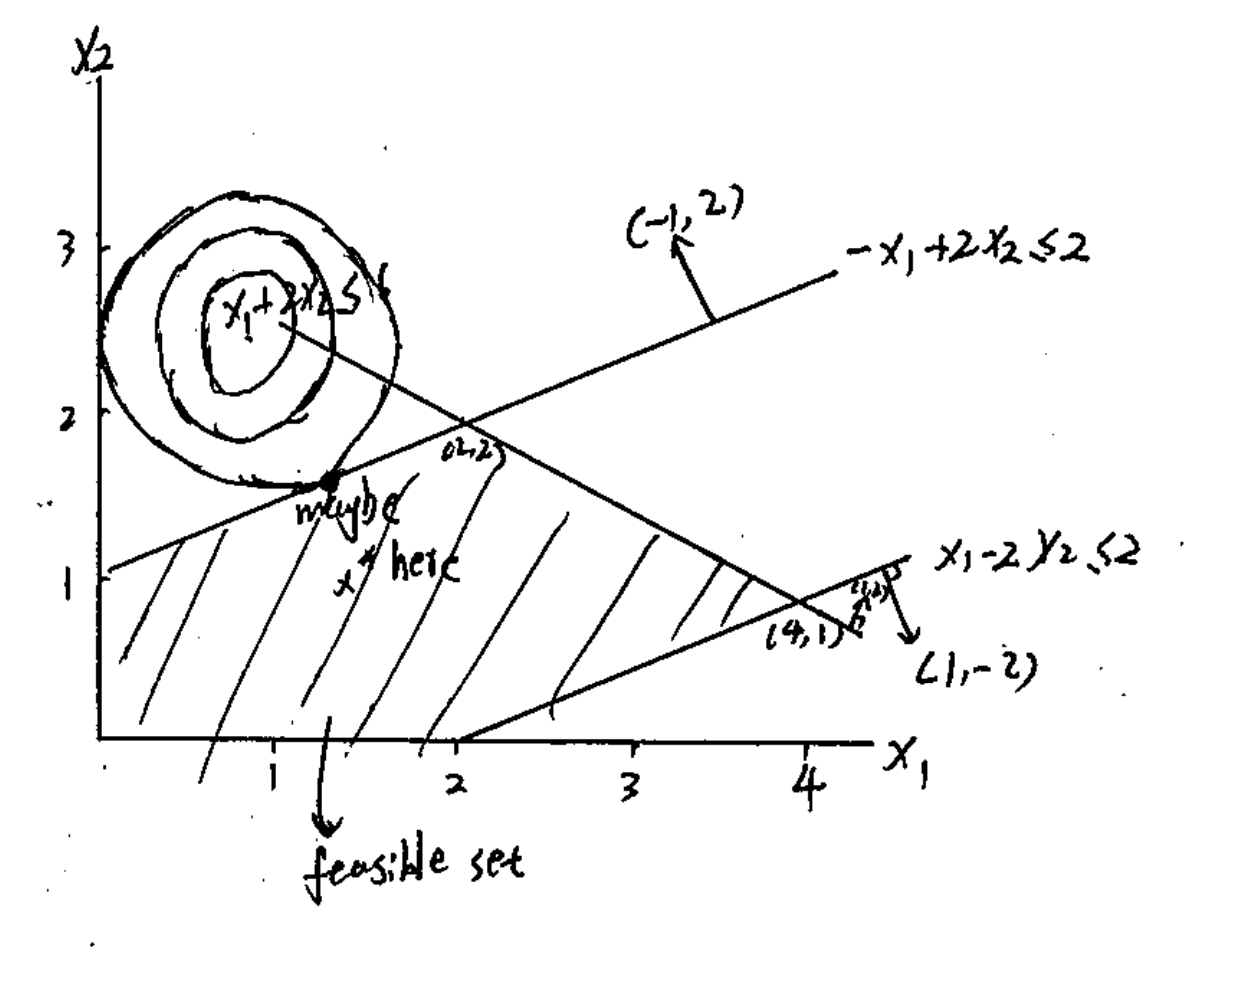
\includegraphics[width=1.8in,height=1.8in]{figures/ch07/figure1021_1.png}
	%\caption{This is an inserted JPG graphic} 
	%\label{fig:graph} 
\end{marginfigure}

\begin{itemize}
	\item at optimum some subset of inequality constraints satisfied with equality "active" set
	
	\item Best "loose"
	
	\item If you know the active set or optimum, just solve an "equality"-constrained QP"
\end{itemize}
By illustrative example:

1) Initialize at $x^{(0)} = \begin{bmatrix}
2\\
0
\end{bmatrix}$, starting with initial "working set" of equality constraint:

\begin{eqnarray}
w_0 = \{x|x_2 = 0 \}
\end{eqnarray}


2) \begin{equation*}
min_{x\in \Re^2} \frac{1}{2}x^T\begin{bmatrix}
2&0\\
0&2
\end{bmatrix}x + \begin{bmatrix}
-2 & -5
\end{bmatrix} + (1 + 2.5^2)
\end{equation*}

s.t. $\begin{bmatrix}
	0  & 1
\end{bmatrix}x = 0$

Recall from last time, we need a basis for $N(\begin{bmatrix}
0\\
1
\end{bmatrix}) = \{x|x = \alpha\begin{bmatrix}
0\\
1
\end{bmatrix} \}$

Say $\begin{bmatrix}
1\\
0
\end{bmatrix} = N\Leftarrow$

\begin{align*}
\tilde{H} &= N^THN = 2\\
\tilde{C} &= (c^TN + \bar{x}HN)\\
&= -2\tilde{d}\\
&= (d+c^Tx + \frac{1}{2}x^THx)
\end{align*}

We convert the problem to :

\begin{align*}
z^* &= argmin\,\,\, z^T\tilde{H}z + \tilde{c}^Tz + \tilde{d}\\
&= argmin\,\,\, \frac{1}{2}2z^2 + (-2z) = \tilde{d}
\end{align*}
 $2z - 2 = 0$, $z = 1$

So the optimum is:

\begin{equation*}
\bar{x}+ z^*N = \begin{bmatrix}
0\\
0
\end{bmatrix} + 1
\begin{bmatrix}
1\\
0
\end{bmatrix} = 
\begin{bmatrix}
1\\
0
\end{bmatrix}
\end{equation*}

Quadratically constrained Quadratic Program:

\begin{align*}
argmin_{x\in \Re^n} &\frac{1}{2}x^THx + c^T + d\\
s.t. &\frac{1}{2}x^TH_ix + c^T_i + d_i \leq 0  & i\in [m]\\
&\frac{1}{2}\tilde{H}_ix + \tilde{c}_i^Tx + \tilde{d}_i = 0 & i\in [q]
\end{align*}

\begin{itemize}
	\item If $H_i = 0, \forall i\in [n]$, $\tilde{H}_i = 0, \forall i\in [q]$, $\rightarrow QP$
	
	\item Typically $h-0\geq 0, H_i\geq 0$, $i\in [m], \tilde{H}_i = o, \forall i\in [q]$. "convex optimization program", set $\tilde{H}_i = 0$
\end{itemize}
Consider a single equality constraint $q = 1$, consider a scalar problem $x\in \Re$:

\begin{equation*}
\tilde{H}_1 = 1 \,\,\, \tilde{c}_i = 0 \,\,\, \tilde{d}_i = -\frac{1}{2}
\end{equation*}

Constraint becomes:

\begin{equation*}
\frac{1}{2}x_1^2 + 0 - \frac{1}{2} = 0\rightarrow x_1^2 = 1
\end{equation*}

Three types of inequality:

Type 1:

\begin{equation*}
H=\begin{bmatrix}
2 &\\
&\frac{1}{2}
\end{bmatrix}\,\,\,c^T = \begin{bmatrix}
0 & 0
\end{bmatrix}\,\,\,
d = -1
\end{equation*}

\begin{align*}
\frac{1}{2}x^THx + c^Tx + d \leq 0\Rightarrow &\frac{1}{2}x^T\begin{bmatrix}
2&\\
&\frac{1}{2}
\end{bmatrix}x\leq 1\\
&x^T\begin{bmatrix}
2&\\
&\frac{1}{2}
\end{bmatrix}x \leq 2
\end{align*}

\begin{align*}
2x_1^2 + \frac{1}{2}x_2^2 &\leq 2\\
x_1 + \frac{1}{4}x_2^2 &\leq 1\\
\frac{x_1^2}{1} + \frac{x_2^2}{4} &\leq 1
\end{align*}
Type 2:

\begin{equation*}
H=0\,\,\,c = \begin{bmatrix}
-1 & 1
\end{bmatrix}\,\,\,
d = -1
\end{equation*}
\begin{equation*}
\begin{bmatrix}
-1 & 1
\end{bmatrix}x\leq 1\Rightarrow
\begin{bmatrix}
-1 & 1
\end{bmatrix}
\begin{bmatrix}
x_1\\
x_2
\end{bmatrix}\leq 1\Rightarrow x_2\leq 1 + x_1
\end{equation*}

\begin{marginfigure}
	\centering
	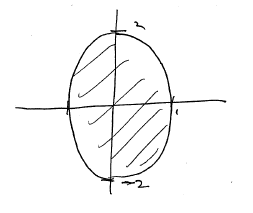
\includegraphics[width=1.8in,height=1.8in]{figures/ch07/figure1021_2.png}
	%\caption{This is an inserted JPG graphic} 
	%\label{fig:graph} 
\end{marginfigure}

Type 3:
\begin{equation*}
H=\begin{bmatrix}
0 &0\\
0&2
\end{bmatrix}\,\,\,c^T = \begin{bmatrix}
-1 & 0
\end{bmatrix}\,\,\,
d = -1 \Rightarrow x^2_2 - x_1 - 1\leq 0
\end{equation*}

\begin{marginfigure}
	\centering
	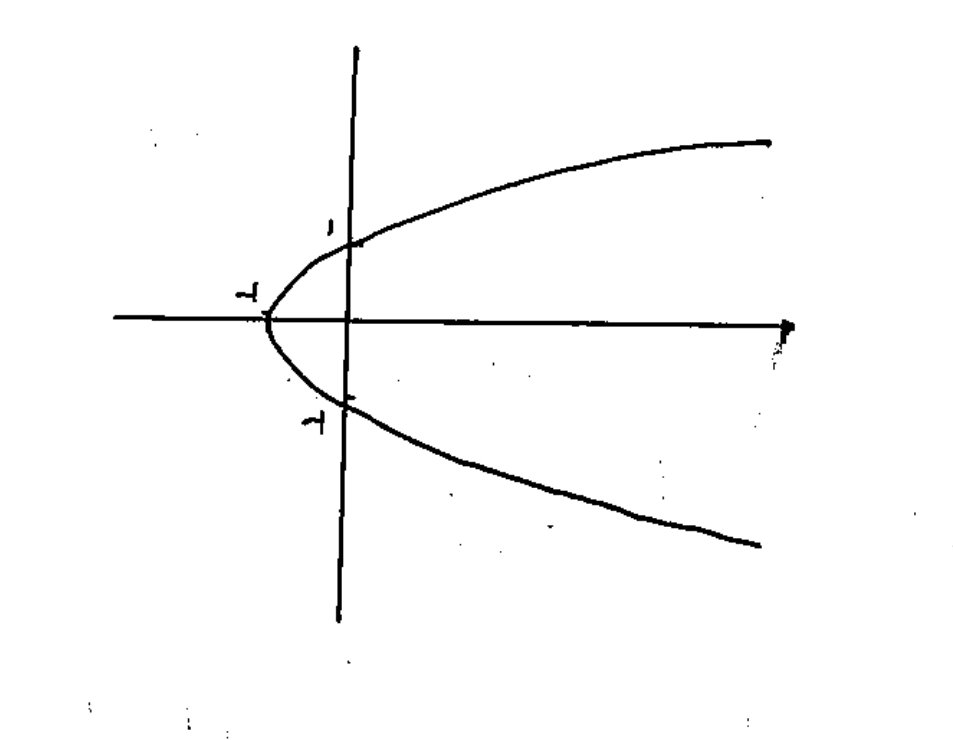
\includegraphics[width=1.8in,height=1.8in]{figures/ch07/figure1021_3.png}
	%\caption{This is an inserted JPG graphic} 
	%\label{fig:graph} 
\end{marginfigure}

Intersection:
\begin{marginfigure}
	\centering
	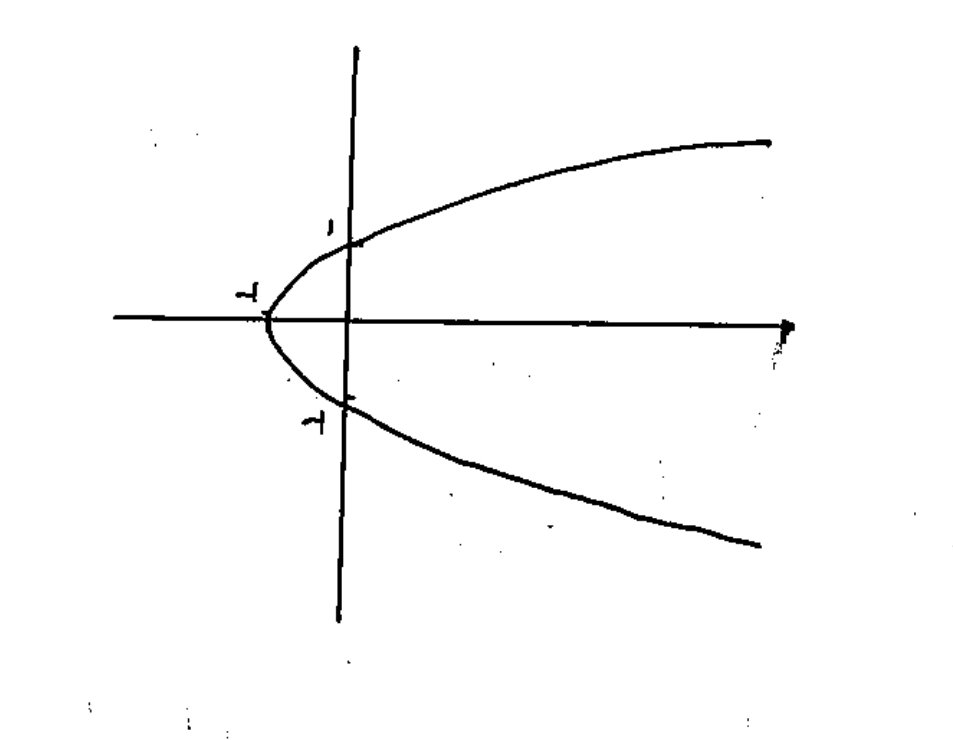
\includegraphics[width=1.8in,height=1.8in]{figures/ch07/figure1021_4.png}
	%\caption{This is an inserted JPG graphic} 
	%\label{fig:graph} 
\end{marginfigure}




%Above are notes for Oct21
